\chapter{Results and Discussion}
\label{cap:Resultados}

This chapter introduces the key findings of this research, beginning with the primary data cleaning and normalization process, which significantly refined the dataset. It analyzes translation quality in open-source LLMs compared to traditional NMT systems for prepositions ACROSS, THROUGH, INTO, and ONTO, categorizing errors and assessing proportions. Additionally, the chapter presents score distribution results for metrics BLUE, METEOR, BERTScore, COMET, and TER, evaluates model performance, and tests the impact of spatial semantics on translation quality. 


\section{Primary Data Cleaning Results}

%M: Antes de apresentar números, lembre aqui rapidamente o que foi feito
%OK
After an extensive data cleaning process involving removal of missing values, duplicates, emojis, incomplete sentences, strange patterns, and rare characters, along with techniques such as length filtering, language detection, and scoring for translation quality, a refined dataset was achieved for NMT translation and evaluation, with a specific focus on spatial prepositions. This refinement significantly enhanced data quality and homogeneity, reducing the initial $610,351$ segments from OPUS datasets to a final dataset of $346,643$ segments, representing a $43\%$ reduction. Table~\ref{tab:cleaning_reasons} outlines the top 10 reasons for segment removal during the cleaning and normalization steps. For the complete breakdown of reasons for segment removal, please refer to Appendix~\ref{app:1} at the end of this document.

\begin{table}[htb]
\centering
\begin{tabular}{lr}
\toprule
\textbf{Reason} & \textbf{Segments} \\
\midrule
Duplicate(s) & $218,427$ \\
Harmful element ``--'' in source or target & $19,343$ \\
Length in tokens is lower than the boundary (4) in source & $7,516$ \\
MTQE score is lower than 0.6 & $5,606$ \\
Length in tokens is lower than the boundary (4) in target & $4,077$ \\
Detected language is not [`pt'] (target) & $2,722$ \\
Harmful element ``['' in source or target & $1,623$ \\ 
Length in characters is higher than the boundary (450) in source & $970$ \\
Possible mismatch (beta) & $716$ \\
Rare character \$ in source or target & $254$ \\
\bottomrule
\end{tabular}
\caption{Reasons for Segment Removal During Data Cleaning.}
\label{tab:cleaning_reasons}
\end{table}

As can be seen in Table~\ref{tab:cleaning_reasons}, the data cleaning process removed a substantial number of segments. Duplicates (duplicated segments) in the corpus constituted the most frequent reason for removal, accounting for a significant portion ($218,427$ segments). Next, segments containing the harmful element ``--'' in either source or target language were removed ($19,343$ segments). This highlights the importance of identifying and eliminating redundant entries and special characters to ensure a unique and representative dataset.

The next two most common reasons for removal were related to sentence length and quality. Segments with a token count (number of words or punctuation marks) less than $4$ in either source or target languages were excluded ($7,516$ and $4,077$ segments, respectively). Additionally, segments with an MTQE score (Machine Translation Quality Estimation score) below $0.6$ were also removed ($5,606$ segments) from the dataset. A lower MTQE score suggests a lower predicted quality of translation, and filtering out these segments helps focus the analysis on higher-quality translations.

Lastly, the remaining entries in Table~\ref{tab:cleaning_reasons} detail the removal of segments for reasons such as length in characters being higher than 450, potential mismatches between source and target lengths, and character `\$' rarity ($970$, $716$, and $254$ segments, respectively).


\section{Score Distribution Results}
\label{sec:Distribution}

In this section, we present the results concerning the distribution of scores across models for the five metrics employed: BLEU, METEOR, BERTScore, COMET, and TER. Analyzing the spread of scores offers valuable insights into performance variation among models. We explore the means, medians, standard deviations, quartile values (Q1 and Q3), delineate the range covered by the whiskers, and compute confidence intervals to achieve a broad understanding of the data distribution and statistical significance among models.


\subsection{BLEU Across Models}

Figure~\ref{fig: blue-models} utilizes BLEU scores to assess model performance. BLEU measures similarity between a generated text and a reference translation by considering \emph{n-}gram precision (how often word sequences match) and a brevity penalty (to avoid overly short outputs). This simple and widely used metric, along with other statistical measures, provides valuable insights into the quality of the text generated by the models.

\begin{figure}[htb]
        \centering        \includegraphics[width=.9\textwidth]{textual/Figuras/Results/unknown-37.png}
        \caption{Distribution of BLEU Across Models..}
        \label{fig: blue-models}
\end{figure}


\subsubsection{Mean and Median}

When comparing the mean (depicted by red circles) and median scores (represented by black lines) in models like Amazon, DeepL, Google, and Mixtral-8x7B, they generally align closely, indicating symmetrical distributions. However, slight differences between means and medians in some LLMs suggest potential effects of outliers in their distributions. Analyzing medians in relation to quartiles offers insights into data spread and model characteristics. For instance, all models consistenly show medians closer to the upper quartile, suggesting that a significant portion of their data falls within higher score ranges.


\subsubsection{Spread of Data}

The interquartile range (IQR), i.e. the difference between the third quartile (Q3) and the first quartile (Q1), serves as a measure of data spread. Models with wider IQRs, such as Amazon, DeepL, and Google, as well as others like Mixtral-8x7B and LLaMa-3-8B, exhibit greater variability compared to those with narrower IQRs, like Mistral-7B, LLaMa-2-7B, and Gemma-7B. Across all models, the lowest whisker is observed close to zero, indicating their lower range, while Amazon (Custom) boasts the highest whisker, nearing $0.942$, indicative of its higher range. Among LLMs, Mixtral-8x7B, LLaMa-3-8B, and LLaMa-2-13B demonstrate wider IQRs, suggesting slightly more variability, whereas LLaMa-2-7B and Gemma-7B exhibit narrower IQRs, indicating more consistent lower performance.


\subsubsection{Outliers}

The presence of outliers, indicated by values beyond the boxplot whiskers (black dots), signifies notable deviations in performance among specific models compared to the dataset. These outliers may represent either exceptionally high or low performance relative to the majority of data points. Specifically, outliers positioned above the upper whisker denote exceptionally high data points, suggesting performance that stands out from the dataset's norm. Among LLMs, models like Gemma-7B and LLaMa-2-7B display the lowest upper-position outliers, implying less variability in their top performance compared to others.


\subsubsection{Confidence Intervals}

The analysis of confidence intervals (CIs) in Table~\ref{tab:mean_ci_scores_blue} provides insights into the precision of mean BLUE score estimates for different models. Models like Google, Gemma-7B, LLaMA-2-7B, LLaMA-2-13B, LLaMA-3-8B, and Mixtral-8x7B have CIs that do not overlap with each other, suggesting potential significant differences in their mean BLUE scores and statistical significance. Conversely, models like Amazon (Custom), Amazon (Stock), and DeepL exhibit overlapping intervals, implying their mean BLUE scores may not be statistically different.

\begin{table}[htb]
\centering
\begin{tabular}{lccc}
\toprule
\textbf{Model} & \textbf{Mean} & \textbf{CIs} & \textbf{SD} \\
\midrule
Amazon (Custom) & $0.370$ & [$0.361$, $0.379$] & $0.1998$ \\
Amazon (Stock) & $\mathbf{0.375}$ & [$0.366$, $0.383$] & $0.1915$ \\
DeepL & $0.366$ & [$0.358$, $0.374$] & $0.1905$ \\
Gemma-7B & $0.011$ & [$0.010$, $0.011$] & $0.0045$ \\
Google & $0.335$ & [$0.327$, $0.343$] & $0.1827$ \\
LLaMA-2-13B & $0.233$ & [$0.226$, $0.240$] & $0.1623$ \\
LLaMA-2-7B & $0.169$ & [$0.163$, $0.175$] & $0.1337$ \\
LLaMA-3-8B & $0.264$ & [$0.257$, $0.271$] & $0.1656$ \\
Mistral-7B & $0.207$ & [$0.200$, $0.213$] & $0.1477$ \\
Mixtral-8x7B & $0.273$ & [$0.266$, $0.280$] & $0.1664$ \\
\bottomrule
\end{tabular}
\caption{Means, Confidence Intervals (CIs), and Standard Deviations (SD) for BLUE scores.}
\label{tab:mean_ci_scores_blue}
\end{table}



\subsection{METEOR Scores Across Models}

Figure~\ref{fig: meteor-models} leverages METEOR scores to provide insights into the quality of text generated by different models. Unlike BLEU, which focuses on \emph{n-}gram precision, METEOR incorporates richer linguistic features like stemming (reducing words to their base form), synonymys, and word order. This design addresses some limitations of BLEU, particularly its sensitivity to minor phrasing differences.

\begin{figure}[htb]
        \centering
        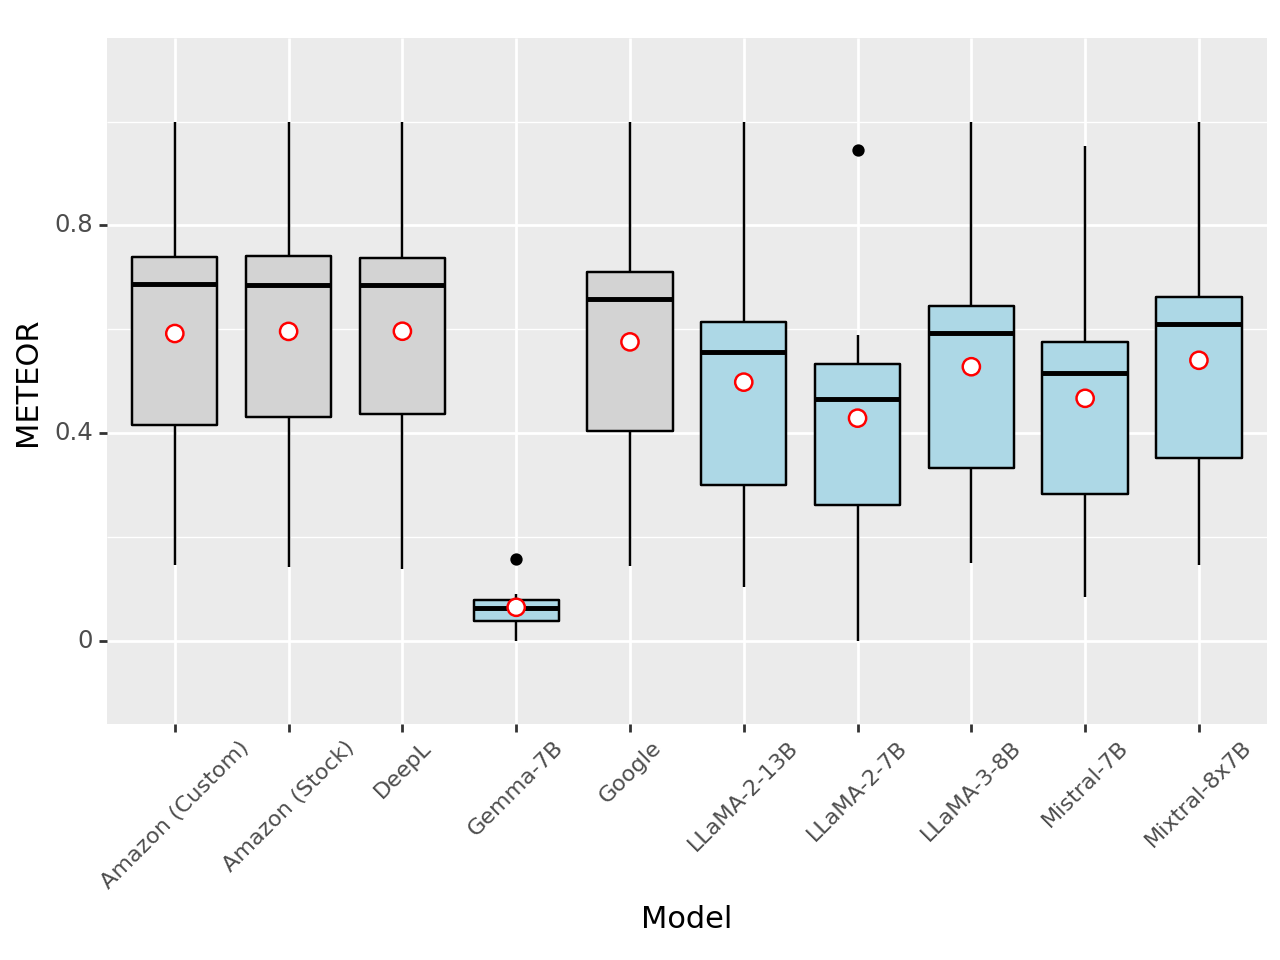
\includegraphics[width=.9\textwidth]{textual/Figuras/Results/Unknown-90.png}
        \caption{Distribution of METEOR Across Models.}
        \label{fig: meteor-models}
\end{figure}


\subsubsection{Mean and median}

When examining the mean (red circles) and median scores (black lines) across METEOR scores for different models, an interesting trend emerges. The mean scores for all models consistently fall a little below the medians, with the medians positioned closer to the upper quartiles, except for Gemma-7B, which shows the mean almost parallel to the median. This pattern suggests that the majority of data points tend to cluster towards higher score ranges, contributing to higher median values. However, the mean scores, possibly influenced by outliers or lower-performing instances, are comparatively lower. This discrepancy indicates potential skewness in the distributions, with some models exhibiting more variability in performance than others.


\subsubsection{Spread of Data}

The IQR (Q3 - Q1) serves as a measure of data dispersion. Across METEOR scores, most models demonstrate similar interquartile sizes, indicating comparable performance variability. Notably, LLaMa-2-7B exhibits a slightly smaller range, while Gemma-7B stands out with a significantly smaller interquartile range, indicating less variability in lower scores. The highest and lowest whiskers in the dataset indicate the range of data distribution among the models. Notably, Gemma-7B and LLaMA-2-7B exhibit the lowest upper whiskers, suggesting a narrower range of performance for these models. Conversely, Google, DeepL and the Amazon models have the highest upper whiskers, indicating a broader spread of performance scores. 

\subsubsection{Outliers}

In Figure~\ref{fig: meteor-models}, only LLaMa-2-7B and Gemma-7B exhibit outliers, marked by black dots above the upper whisker. These outliers indicate significant deviations in performance compared to the bulk of the data, representing exceptionally high scores relative to the majority of data points. Despite their lower scores, Gemma-7B and LLaMa-2-7B stand out as outliers due to the limited number of displayed outliers in the plot.


\subsubsection{Confidence Intervals}

The analysis of CIs for METEOR scores reveals valuable insights into the statistical significance of differences in mean performance across various models. Upon examination of Table~\ref{tab:mean_ci_scores_meteor}, it is evident that the intervals for Amazon (Custom), Amazon (Stock), and DeepL overlap with each other, suggesting that their mean METEOR scores may not be statistically different from one another. On the other hand, the intervals for Gemma-7B, LLaMA-2-13B, LLaMA-3-8B, Mistral-7B, and Mixtral-8x7B do not overlap with those of any other model, indicating potential statistical significance in their performance. 

\begin{table}[htb]
\centering
\begin{tabular}{lccc}
\toprule
\textbf{Model} & \textbf{Mean} & \textbf{CIs} & \textbf{SD} \\
\midrule
Amazon (Custom) & $\mathbf{0.687}$ & [$0.680$, $0.693$] & $0.1468$ \\
Amazon (Stock) & $0.686$ & [$0.679$, $0.693$] & $0.1434$ \\
DeepL & $0.685$ & [$0.679$, $0.692$] & $0.1392$ \\
Gemma-7B & $0.067$ & [$0.066$, $0.068$] & $0.0298$ \\
Google & $0.659$ & [$0.652$, $0.665$] & $0.1440$ \\
LLaMA-2-13B & $0.559$ & [$0.552$, $0.566$] & $0.1596$ \\
LLaMA-2-7B & $0.467$ & [$0.459$, $0.474$] & $0.1730$ \\
LLaMA-3-8B & $0.593$ & [$0.587$, $0.600$] & $0.1495$ \\
Mistral-7B & $0.515$ & [$0.508$, $0.522$] & $0.1556$ \\
Mixtral-8x7B & $0.610$ & [$0.604$, $0.617$] & $0.1461$ \\
\bottomrule
\end{tabular}
\caption{Means, Confidence Intervals (CIs), and Standard Deviations (SD) for METEOR scores.}
\label{tab:mean_ci_scores_meteor}
\end{table}


\subsection{BERTScore Across Models}

Figure~\ref{fig: bertscore-models} depicts model performance using BERTScores. Alongside other statistical measures, these scores offer insights into the quality of the text generated by these models. Unlike metrics like BLEU or METEOR, BERTScore utilizes contextual embeddings from BERT to assess semantic similarity between a generated sentence (candidate) and a reference sentence. By considering contextual information, BERTScore potentially provides more nuanced evaluation. %M: Descrição muito sumária. Coloque ao menos 2 ou 3 linhas explicando em que o BERTscore difere do Meteor. Isso tem de ser feito para todas as métricas. Do contrário, você vai perder o entendimento do leitor.

\begin{figure}[htb]
        \centering
        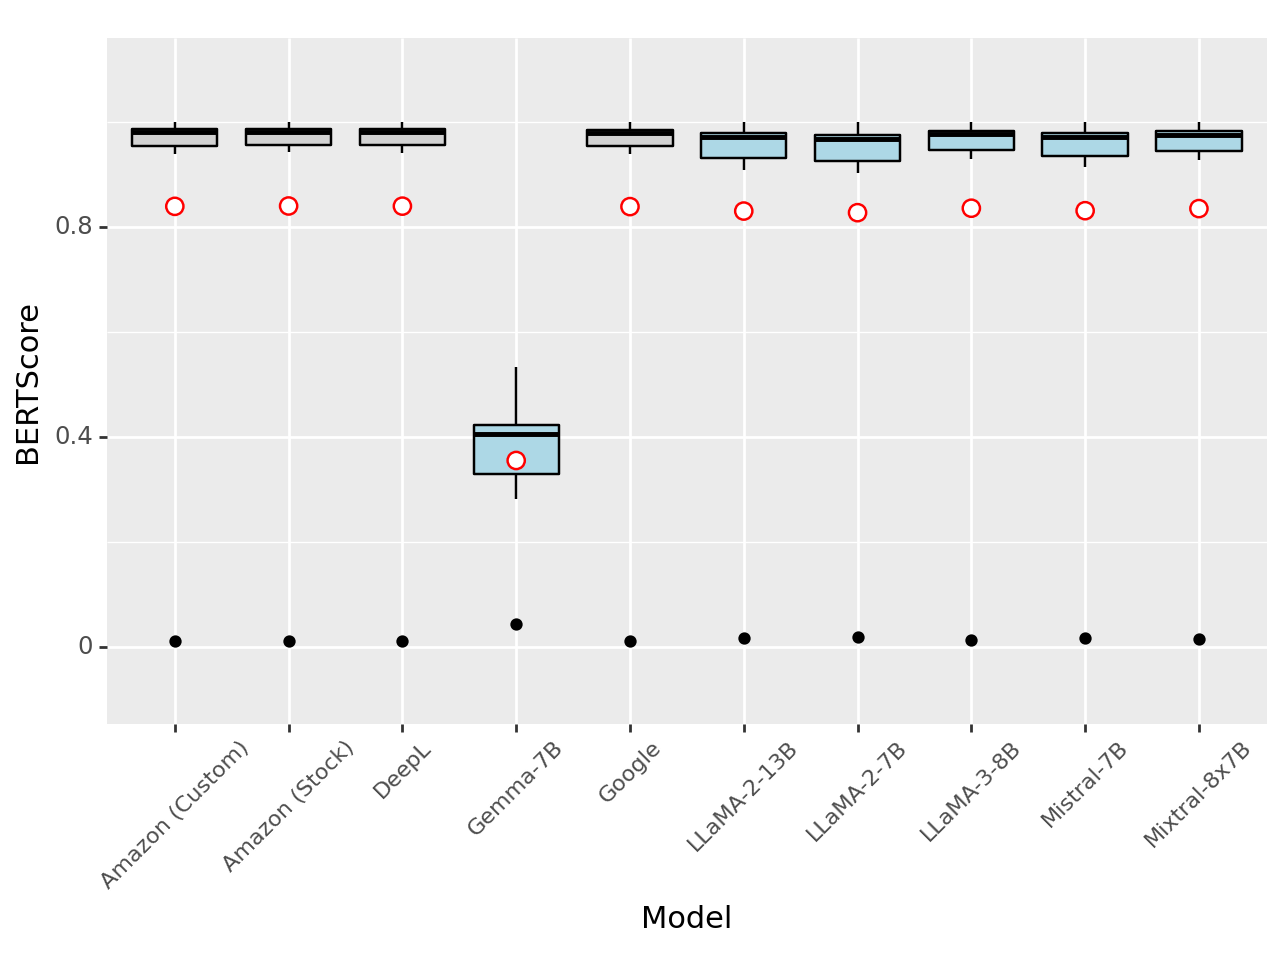
\includegraphics[width=.9\textwidth]{textual/Figuras/Results/Unknown-93.png}
        \caption{Distribution of BERTScore Across Models.}
        \label{fig: bertscore-models}
\end{figure}

        
\subsubsection{Mean and Median}

When comparing the mean (red circles) and median scores (black lines) for BERTScore across different models, noticeable patterns emerge. In most cases, the mean values fall outside the boxplots towards the lower bound, potentially influenced by lower-bound outliers close to zero. This suggests that some outlier data points significantly affect the mean, pulling it towards the lower end of the distribution. Conversely, the medians are consistently positioned very close to the upper quartile bound, indicating that the central tendency of the data lies towards higher score ranges. However, Gemma-7B stands out, with both the mean and median positioned inside the quartile. Interestingly, Gemma-7B's mean is closer to the lower quartile, suggesting a distribution skewed towards lower scores compared to other models.


\subsubsection{Spread of Data}

The IQRs (Q3 -- Q1) provide insights into the spread of data. Gemma-7B stands out with the largest interquartile range compared to other models, despite its lower scores, indicating higher variability in its performance. Conversely, the interquartile ranges for all other models are relatively small and close to 1, suggesting minimal variability in their performance scores. This consistency in interquartile sizes near 1 indicates that the majority of data points for these models fall within a narrow range of scores, contributing to a more consistent performance across different inputs. However, while this highlights consistency, it may also suggest a lack of significant variation among models in terms of their best performance.


\subsubsection{Outliers}

As already discussed, the presence of outliers very close to zero in all models, as seen in Figure~\ref{fig: bertscore-models}, significantly impacts their mean scores, pulling them downwards. These outliers highlight instances where the models struggle with certain inputs, indicating potential challenges in translation accuracy. Addressing these outliers is crucial for enhancing the models' reliability and performance consistency across various inputs and scenarios.


\subsubsection{Confidence Intervals}

The analysis of CIs for BertScore scores reveals notable patterns in mean performance across various models. Overlapping CIs observed among Amazon (Custom), Amazon (Stock), DeepL, and Google, as well as between LLaMA-2-13B and Mistral-7B, and LLaMA-3-8B and Mixtral-8x7B, suggest similar mean BertScore scores. Conversely, non-overlapping intervals for Gemma-7B and LLaMa-2-7B and indicate potential significant differences in their mean BertScore scores compared to other models. These findings underscore the statistical significance of performance variations and emphasize the importance of considering CIs when interpreting BertScore evaluations.

\begin{table}[htb]
\centering
\begin{tabular}{lccc}
\toprule
\textbf{Model} & \textbf{Mean} & \textbf{CIs} & \textbf{SD} \\
\midrule
Amazon (Custom) & $\mathbf{0.980}$ & [$0.979$, $0.981$] & $0.012$ \\
Amazon (Stock) & $\mathbf{0.980}$ & [$0.980$, $0.981$] & $0.012$ \\
DeepL & $\mathbf{0.980}$ & [$0.979$, $0.981$] & $0.012$ \\
Gemma-7B & $0.407$ & [$0.405$, $0.409$] & $0.045$ \\
Google & $0.979$ & [$0.978$, $0.980$] & $0.013$ \\
LLaMA-2-13B & $0.971$ & [$0.970$, $0.972$] & $0.018$ \\
LLaMA-2-7B & $0.966$ & [$0.965$, $0.967$] & $0.020$ \\
LLaMA-3-8B & $0.975$ & [$0.975$, $0.976$] & $0.015$ \\
Mistral-7B & $0.970$ & [$0.969$, $0.971$] & $0.018$ \\
Mixtral-8x7B & $0.974$ & [$0.974$, $0.975$] & $0.015$ \\
\bottomrule
\end{tabular}
\caption{Means, Confidence Intervals (CIs), and Standard Deviations (SD) for BERTScores.}
\label{tab:mean_ci_scores_bert}
\end{table}


\subsection{COMET Across Models}

Figure~\ref{fig: comet-models} utilizes COMET scores to assess the quality of text generated by different models. Unlike metrics like BLEU or METEOR, which focus on \emph{n}-gram overlap, COMET is specifically designed for evaluating translations in conversational contexts. It achieves this by considering various aspects of language important in conversation, such as fluency, relevance, and specificity. To make these judgments, COMET employs pre-trained models.

\begin{figure}[htb]
        \centering
        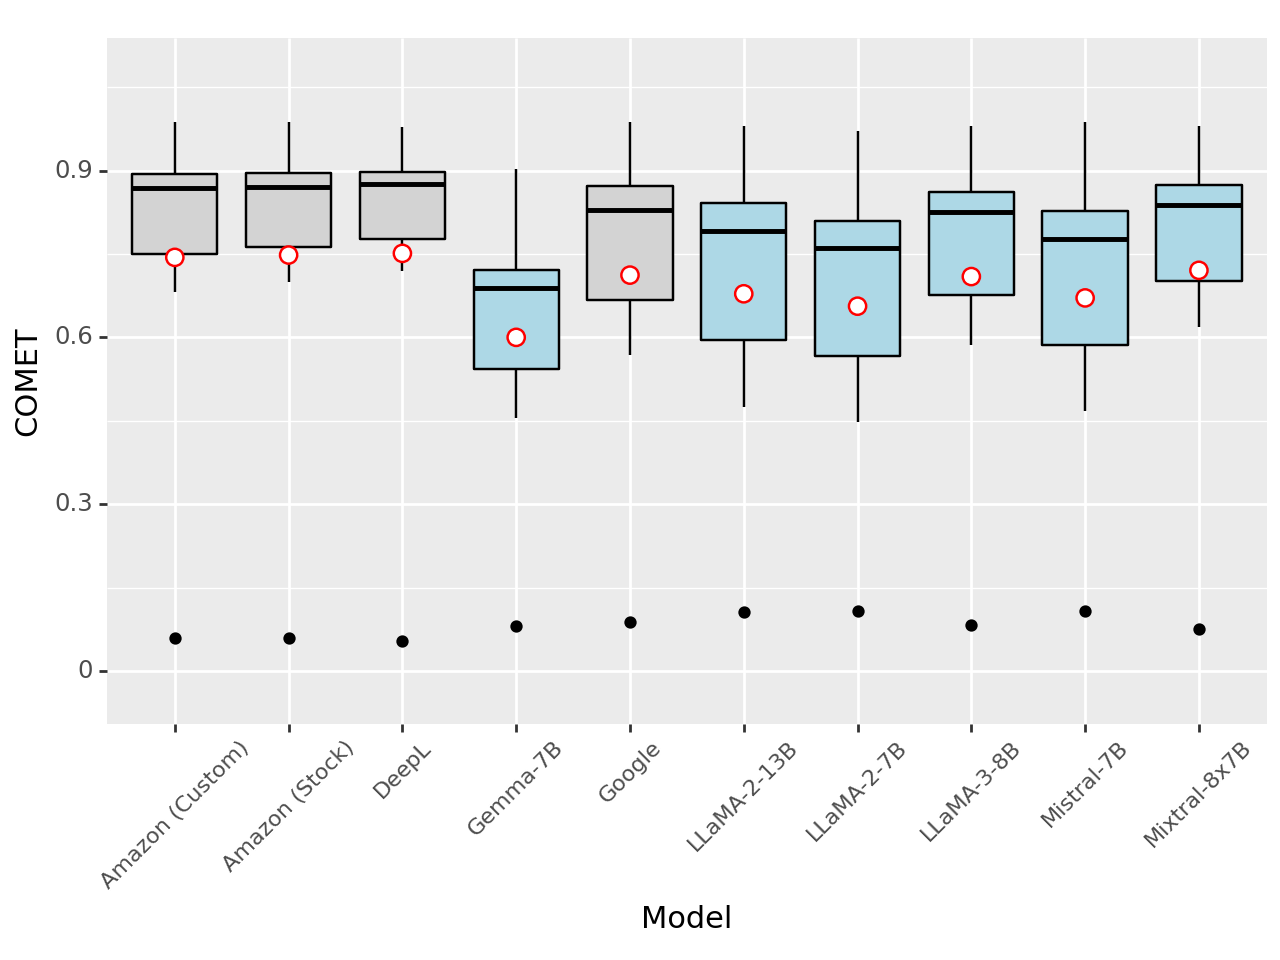
\includegraphics[width=.9\textwidth]{textual/Figuras/Results/Unknown-94.png}
        \caption{Distribution of COMET Across Models.}
        \label{fig: comet-models}
\end{figure}


\subsubsection{Mean and Median}

The analysis of means and medians reveals a consistent trend across models, with medians (black lines) consistently positioned near the upper quartile, indicating a concentration of data in higher score ranges. However, the means (red circles) vary among models, some appearing very close to the lower quartile, such as Google, Mixtral-8x7B, and LLaMa-3-8B, while others fall slightly outside the interquartile range, notably observed in the Amazon models and DeepL. This suggests potential negative skewness in certain distributions and underscores the importance of carefully considering outlier effects in data analysis.


\subsubsection{Spread of Data}

Analyzing the spread of data and interquartile ranges (Q3 - Q1) across models provides insights into the variability of COMET scores. The interquartile ranges vary less across models, indicating similarities in data spread and performance consistency. Among NMT providers, Amazon and DeepL exhibit overlapping interquartile ranges, suggesting similarity in performance, while Google shows more variability. Interestingly, among LLMs, Mixtral-8x7B and LLaMa-3-8B present overlaps with Google, suggesting similarities in score distributions. Conversely, Gemma-7B displays the lowest-positioned interquartile range, indicating more consistent performance, but with lower scores.


\subsubsection{Outliers}

The existence of outliers, as depicted in Figure~\ref{fig: comet-models}, substantially influences the mean scores, causing them to decrease. These outliers indicate situations where the models encounter difficulties with specific inputs, suggesting potential challenges in translation accuracy. It is essential to address these outliers to improve the reliability and consistency of the models' performance across different inputs and scenarios.


\subsubsection{Confidence Intervals}

The examination of CIs offers valuable insights into the statistical significance of performance differences among models. Referring to Table~\ref{tab:mean_ci_scores_comet}, it becomes apparent that the intervals for LLaMA-3-8B and Google, along with those for Amazon (Stock) and Amazon (Custom), overlap. This overlap suggests that the mean scores of these models may not exhibit statistically significant differences. Conversely, Gemma-7B, LLaMA-2-13B, LLaMA-3-8B, Mistral-7B, and Mixtral-8x7B show non-overlapping confidence intervals, indicating potential significant distinctions in their mean scores. 

\begin{table}[htb]
\centering
\begin{tabular}{lccc}
\toprule
\textbf{Model} & \textbf{Mean} & \textbf{CIs} & \textbf{SD} \\
\midrule
Amazon (Custom) & $0.870$ & [$0.869$, $0.871$] & $0.059$ \\
Amazon (Stock) & $0.871$ & [$0.868$, $0.874$] & $0.058$ \\
DeepL & $\mathbf{0.875}$ & [$0.873$, $0.878$] & $0.053$ \\
Gemma-7B & $0.688$ & [$0.685$, $0.692$] & $0.081$ \\
Google & $0.830$ & [$0.826$, $0.834$] & $0.088$ \\
LLaMA-2-13B & $0.791$ & [$0.787$, $0.796$] & $0.107$ \\
LLaMA-2-7B & $0.761$ & [$0.757$, $0.766$] & $0.108$ \\
LLaMA-3-8B & $0.826$ & [$0.822$, $0.830$] & $0.081$ \\
Mistral-7B & $0.777$ & [$0.773$, $0.781$] & $0.107$ \\
Mixtral-8x7B & $0.840$ & [$0.837$, $0.842$] & $0.075$ \\
\bottomrule
\end{tabular}
\caption{Means, Confidence Intervals (CIs), and Standard Deviations (SD) for COMET scores.}
\label{tab:mean_ci_scores_comet}
\end{table}


\subsection{TER Across Models}

Figure~\ref{fig: ter-models} depicts model performance based on TER scores. These scores, combined with other statistical measures, provide insights into the quality of text generated by the models. Unlike metrics that focus on similarity (BLEU, METEOR) or contextual understanding (BERTScore, COMET), TER takes a different approach. It measures the number of edits required to transform a machine translation into a reference translation. This simple and efficient method, however, has limitations. TER struggles to capture semantic differences between the original text and the translations, potentially overlooking quality issues.

\begin{figure}[htb]
        \centering
        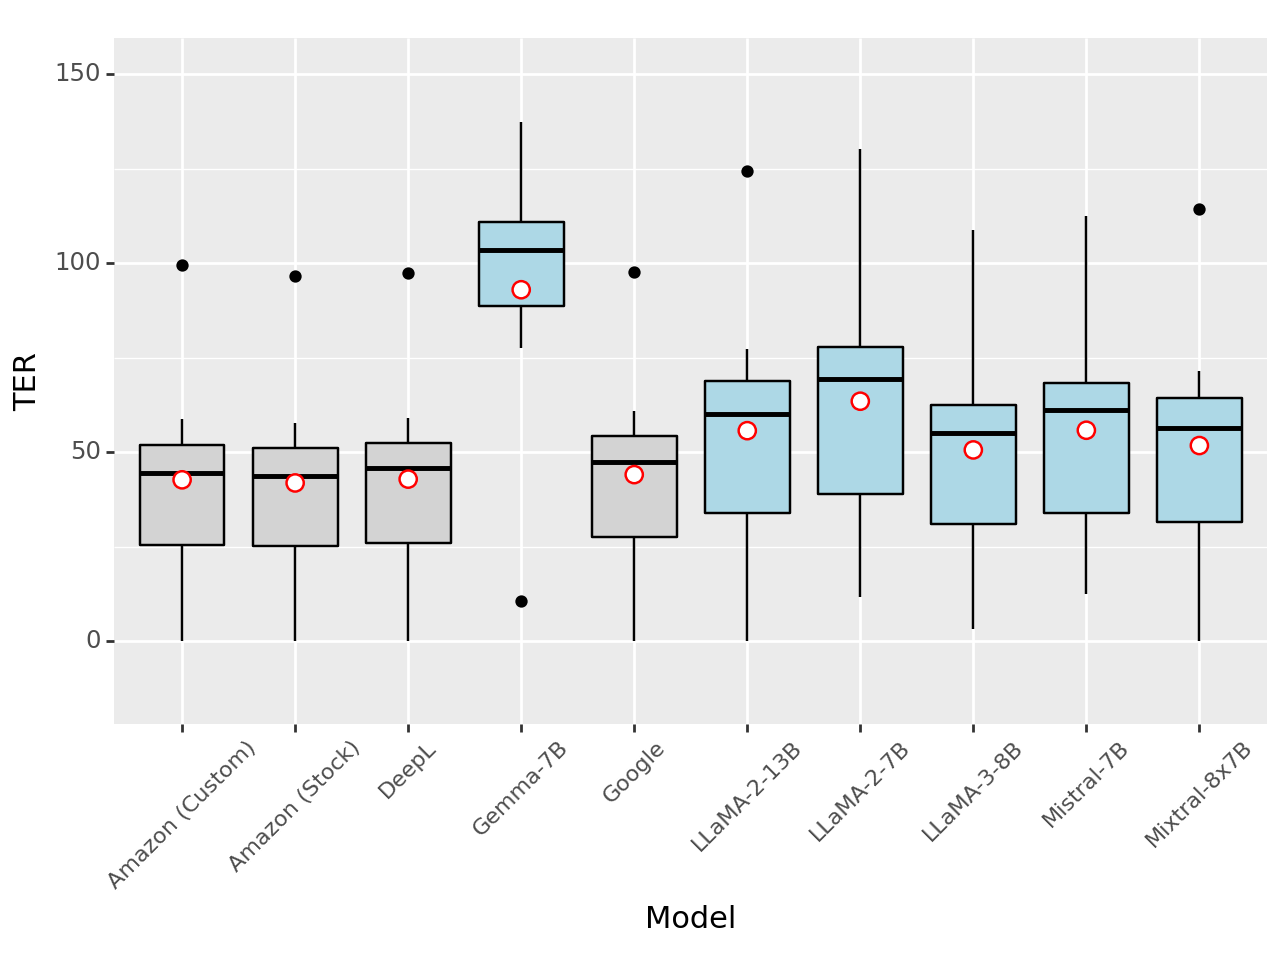
\includegraphics[width=.9\textwidth]{textual/Figuras/Results/Unknown-95.png}
        \caption{Distribution of TER Across Models.}
        \label{fig: ter-models}
\end{figure}
        

\subsubsection{Mean and Median}

The analysis of mean and median scores highlights a consistent trend observed across models, with medians (represented by black lines) consistently situated near the upper quartile. This implies a concentration of data in higher score ranges. However, the influence of outliers on means (depicted by red circles) varies across models, pulling them either very close to the median and upper quartile, as seen in most models, or to the lower quartile, particularly noticeable in Gemma-7B. This suggests potential negative skewness in certain distributions, highlighting the need for careful consideration of outlier effects in data analysis.


\subsubsection{Spread of Data}

The IQR, calculated as Q3 - Q1, provides insight into the spread of data within the middle 50\% of observations. Models like LLaMA-2-13B, LLaMA-2-7B, and Mistral-7B have wider IQRs (around $31.337$, $29.641$, and $25.000$ respectively), suggesting more variability in their TER scores. Conversely, models such as Gemma-7B have narrower IQRs (around $15.000$), indicating less variability. Gemma-7B as well as LLaMA-2-7B exhibit the highest whisker values (around $137.500$ and $130.175$ respectively), implying higher scores, which in this case means lower performance compared to the other models. Conversely, LLaMA-2-7B has the lowest whisker values (around $0.00$). These extreme values highlight potentially influential data points beyond the quartiles.


\subsubsection{Outliers}

As depicted in Figure~\ref{fig: ter-models}, outliers noticeably affect model performance assessment in the dataset. Across most models, outliers tend to elevate the mean TER scores closer to the upper quartile, indicating higher translation errors. However, in Gemma-7B, outliers pull the mean TER score closer to the lower quartile, suggesting unusually low translation errors, which in this case mean good translations. This disparity underscores the diverse impact of outliers on model evaluation, highlighting the complexity of interpreting model performance amidst the presence of outliers.


\subsubsection{Confidence Intervals}

Analyzing mean TER scores and their confidence intervals reveals patterns of overlap and distinctiveness among models, as illustrated in Table~\ref{tab:mean_ci_scores_ter}. LLaMA-3-8B and Mixtral-8x7B, as well as other pairs such as Amazon (Custom) and Amazon (Stock), and Mistral-7B and LLaMA-2-13B, demonstrate overlapping confidence intervals, suggesting potential similarity in their performance. Conversely, Gemma-7B and LLaMA-2-7B exhibit distinct intervals, hinting at differences in their mean TER scores. Particularly, Gemma-7B stands out with a notably higher mean and non-overlapping interval, indicating the lowest performance and potential statistical significance compared to other models.

\begin{table}[htb]
\centering
\begin{tabular}{lccc}
\toprule
\textbf{Model} & \textbf{Mean} & \textbf{CIs} & \textbf{SD} \\
\midrule
Amazon (Custom) & $44.709$ & [$43.850$, $45.569$] & $19.257$ \\
Amazon (Stock) & $\mathbf{44.438}$ & [$43.612$, $45.265$] & $18.621$ \\
DeepL & $45.676$ & [$44.844$, $46.508$] & $18.678$ \\
Gemma-7B & $106.799$ & [$106.319$, $107.278$] & $10.663$ \\
Google & $47.501$ & [$46.676$, $48.327$] & $18.508$ \\
LLaMA-2-13B & $60.403$ & [$59.414$, $61.392$] & $21.803$ \\
LLaMA-2-7B & $69.953$ & [$68.986$, $70.919$] & $21.510$ \\
LLaMA-3-8B & $55.700$ & [$54.855$, $56.546$] & $18.963$ \\
Mistral-7B & $61.271$ & [$60.481$, $62.062$] & $17.651$ \\
Mixtral-8x7B & $56.251$ & [$55.345$, $57.157$] & $20.176$ \\
\bottomrule
\end{tabular}
\caption{Means, Confidence Intervals (CIs), and Standard Deviations (SD) for TER scores.}
\label{tab:mean_ci_scores_ter}
\end{table}



\section{Manual Error Analysis}
\label{sec: Error-analysis}

In this section, we present the results of the human evaluation step. As described in Section~\ref{sec: Human Evaluation}, 10\% of the data (200 segments) were randomly selected for manual error classification. The labels used for error categorization were described in Table~\ref{tab: error_categories}.


\subsection{Analysis by Model: Correct Translations vs. Errors}

Models were initially evaluated based on their overall ability to produce correct translations while minimizing errors. Table~\ref{tab:corrects_errors_summary} provides a summary of the total of correct translations and errors for different models. Here, this analysis helps us understand how different LLMs performed individually and compared to traditional NMT systems.

\begin{table}[htb]
\centering
\begin{tabular}{lcccc}
\toprule
& \multicolumn{2}{c}{\textbf{Total of}} & \multicolumn{2}{c}{\textbf{\% of}} \\
\cmidrule(lr){2-3} \cmidrule(lr){4-5}
\textbf{Model} & \textbf{CC} & \textbf{ER} & \textbf{CC} & \textbf{ER} \\
\midrule
DeepL & $156$ & $44$ & $78.00\%$ & $22.00\%$ \\
\midrule
Gemma-7B & $46$ & $282$ & $14.02\%$ & $85.98\%$ \\
LLaMA-2-13B & $26$ & $333$ & $7.24\%$ & $92.76\%$ \\
LLaMA-2-7B & $19$ & $\mathbf{421}$ & $4.31\%$ & $95.68\%$ \\
LLaMA-3-8B & $45$ & $232$ & $16.25\%$ & $83.75\%$ \\
Mistral-7B & $16$ & $374$ & $4.10\%$ & $\mathbf{95.90\%}$ \\
Mixtral-8x7B & $\mathbf{71}$ & $177$ & $\mathbf{28.63}\%$ & $71.37\%$ \\
\bottomrule
\end{tabular}
\caption{Summary of Correct Translations (CC) vs. Errors (ER) by Model.}
\label{tab:corrects_errors_summary}
\end{table}


The analysis of correct translations vs. errors reveals that DeepL, an NMT system, significantly outperformed all LLMs, achieving $156$ ($78\%$) correct translations and $44$ ($22\%$) errors. Among LLMs, Mixtral-8x7B demonstrated the best performance with $71$ ($\approx29\%$) correct translations and $177$ ($\approx71\%$) errors. Gemma-7B and LLaMA-3-8B exhibited the second and third highest performance, with $46$ ($\approx14\%$) and $45$ ($\approx16\%$) correct translations, respectively. Notably, Gemma-7B had considerably more errors than LLaMA-3-8B, with $50$ ($2.26\%$) more errors. Meanwhile, LLaMA-2-13B, LLaMA-2-7B, and Mistral-7B showed the lowest performance, with correct translation percentages ranging from $\approx4\%$ to $\approx16\%$. Particularly, Mistral-7B presented the highest proportion of errors ($\approx96\%$) among LLMs. We emphasize that a `correct' translation does not contain errors of any type. In Table~\ref{tab:corrects_errors_summary}, values in bold indicate the models with the best and worst performance among the LLMs. This analysis emphasizes the need for further improvement in LLMs to compete with traditional NMT systems in terms of translation accuracy.


\subsection{Analysis by Model: Spatial vs. Non-spatial \& Other Errors}

Models were then assessed based on subgroups of error types to gain a better understanding of the relationship between different models and specific types of errors. Table~\ref{tab:model_performance_by_error_type} provides a summary of the number of errors grouped into spatial, non-spatial, and other categories.

\begin{table}[htb]
\centering
\begin{tabular}{lcccccc}
\toprule
& \multicolumn{3}{c}{\textbf{Total of Errors}} & \multicolumn{3}{c}{\textbf{\% of Errors}} \\
\cmidrule(lr){2-4} \cmidrule(lr){5-7}
\textbf{Model} & \textbf{SP} & \textbf{N-SP} & \textbf{OE} & \textbf{SP} & \textbf{N-SP} & \textbf{OE} \\
\midrule
DeepL & $8$ & $13$ & $23$ & $\mathbf{21.62\%}$ & $\mathbf{35.14}\%$ & $43.24\%$ \\
\midrule
Gemma-7B & $11$ & $25$ & $246$ & $4.09\%$ & $9.29\%$ & $86.62\%$ \\
LLaMA-2-13B & $16$ & $32$ & $285$ & $6.19\%$ & $7.71\%$ & $86.10\%$ \\
LLaMA-2-7B & $\mathbf{25}$ & $31$ & $365$ & $4.17\%$ & $5.17\%$ & $\mathbf{90.67\%}$ \\
LLaMA-3-8B & $18$ & $31$ & $183$ & $5.36\%$ & $10.77\%$ & $83.87\%$ \\
Mistral-7B & $20$ & $\mathbf{38}$ & $\mathbf{316}$ & $5.33\%$ & $10.11\%$ & $84.56\%$ \\
Mixtral-8x7B & $17$ & $30$ & $130$ & $\mathbf{9.14\%}$ & $\mathbf{16.13\%}$ & $74.73\%$ \\
\bottomrule
\end{tabular}
\caption{Comparison of Spatial (SP) vs. Non-spatial (N-SP) and Other Errors (OE) by Model.}
\label{tab:model_performance_by_error_type}
\end{table}

The analysis of Table~\ref{tab:model_performance_by_error_type} reveals a complex relationship between models and error categories. While a strong correlation between model robustness and overall performance might be expected, a closer look is needed. Examining the table, we can observe a trend where LLMs tend to have a predominance of non-spatial errors and a considerably higher number of other errors compared to DeepL. For instance, Mistra-7B had the biggest number of non-spatail errors ($38$), as well as other errors ($316$), while the biggest proportions were obtained by DeepL, with $\approx35\%$, and LLaMa-2-7B, with  $1\approx91\%$.

The table also reveals a variation in the total number of spatial errors across models. DeepL, the only NMT system, despite having the fewest number ($8$), has the highest proportion ($\approx22\%$) of spatial errors. This means that its relatively small number of spatial errors affected model performance more compared to LLMs. Conversely, among LLMs, LLaMA-2-7B has the lowest proportion ($\approx5\%$), followed by LLaMA-2-13B with $\approx8\%$. Interestingly, Mixtral-8x7B did not vary considerably between spatial and non-spatial errors but showed the best performance in handling other errors, with $130$ ($\approx75\%$).

These findings suggest a potential trend: current open-source LLMs might be more susceptible to translation errors in general, including both spatial and non-spatial errors, compared to NMT systems. Even when some LLMs have similar total error rates, a closer look reveals a bias towards non-spatial errors. This underlines the importance of considering error proportions, not just total error count, for a comprehensive evaluation of model performance.


\subsection{Analysis by Model: Exploring All Error Types}

Taking the analysis a step further, we examine whether different models exhibit a propensity for specific error types. Figure~\ref{fig: error-types} provides a detailed breakdown of the total number of specific errors types by model (please, refer back to Table~\ref{tab: error_categories} for the complete description of error categories). Our aim is to identify potential patterns in error distribution across models to gain a deeper understanding of their strengths and weaknesses.

\begin{figure}[htb]
        \centering
        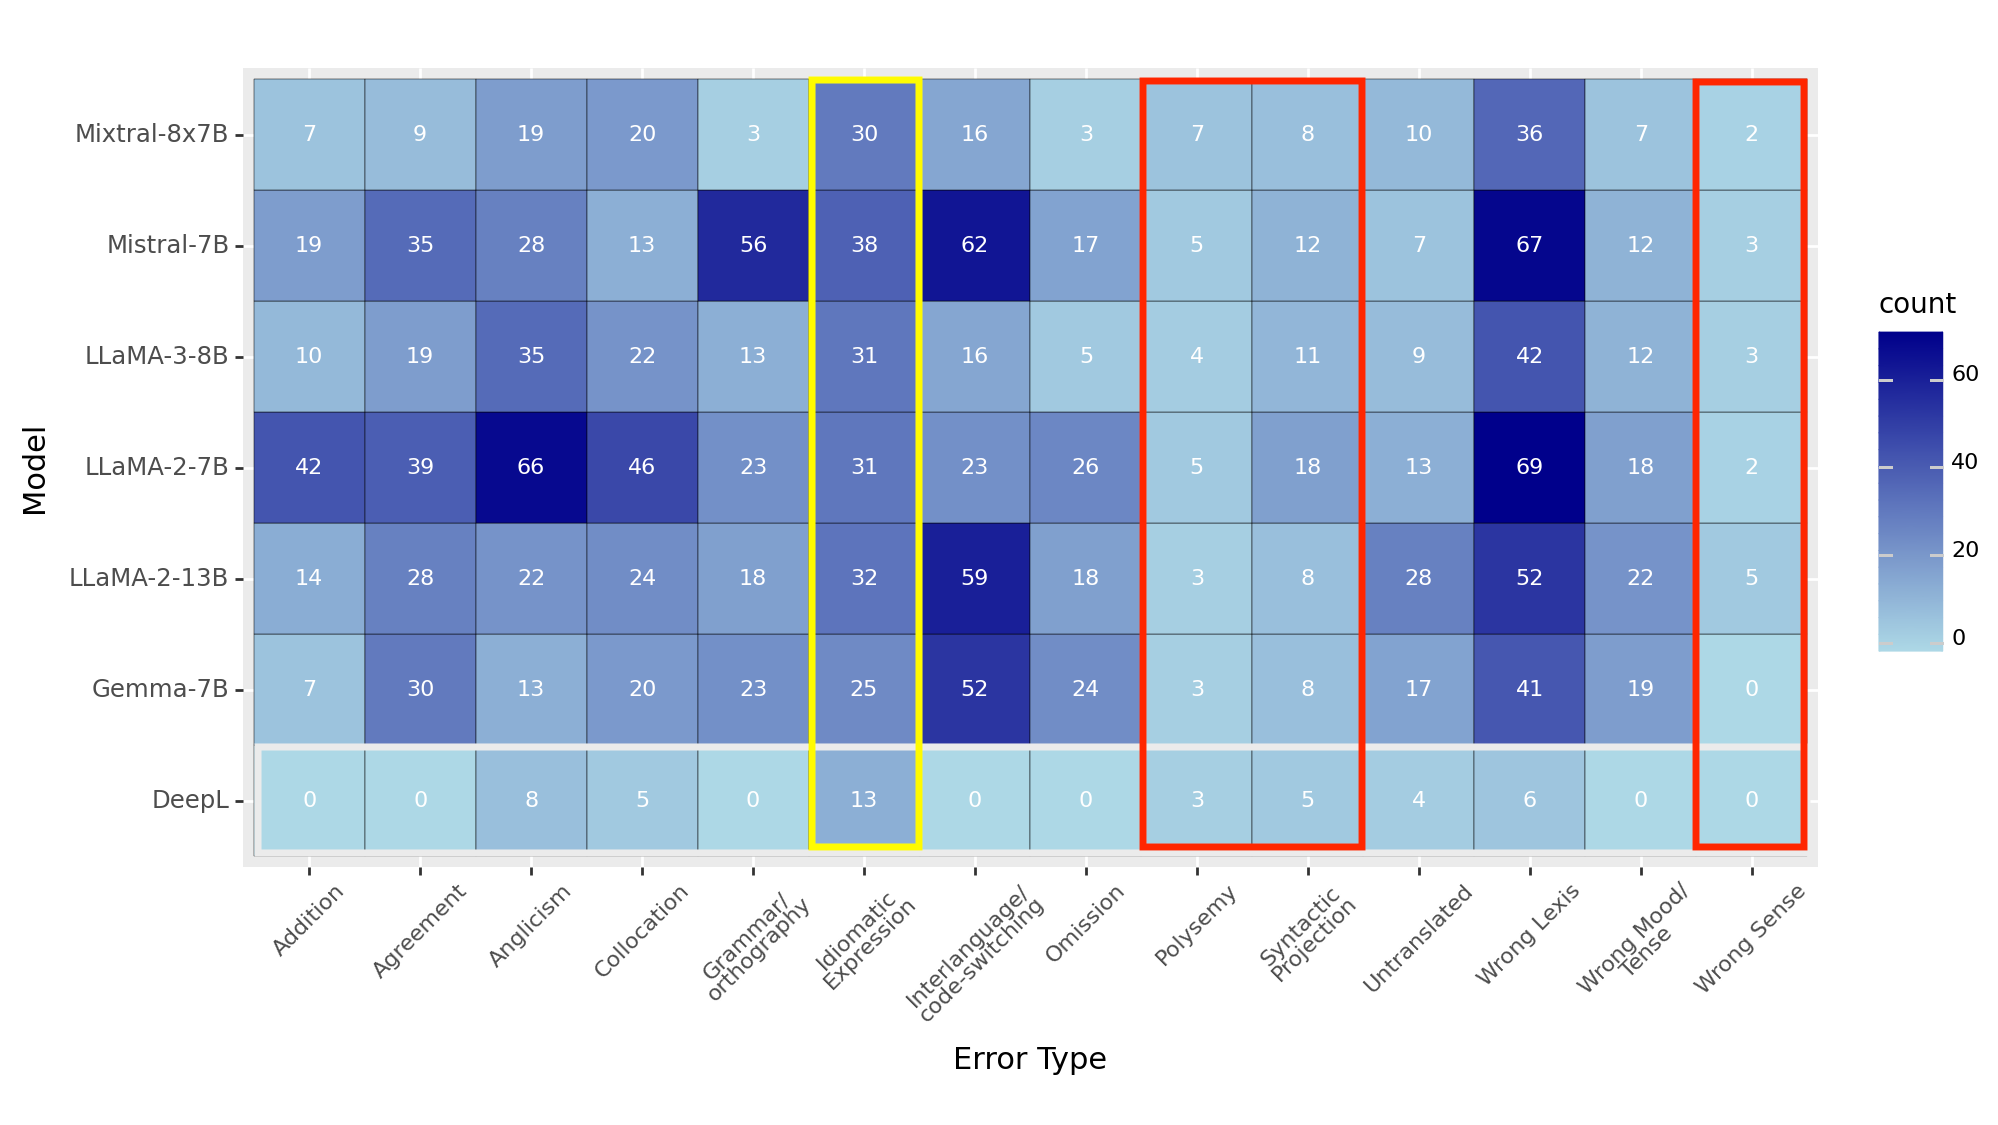
\includegraphics[width=1\textwidth]{textual/Figuras/Results/Unknown-44.png}
        \caption{Distribution of All Error Types by Model (Count).}
        \label{fig: error-types}
\end{figure}

The heatmap in Figure~\ref{fig: error-types} offers insights into the distribution of general and spatial errors across various models. As delineated in Subsection~\ref{subsec: Manual Error Classification}, spatial errors (highlighted in red), the core of our investigation, encompass polysemy (po), syntactic projection (sp), and wrong sense (ws). Additionally, our focus extends to examining idiomatic expression (ie) errors (highlighted in yellow). DeepL (highlighted in white) was the only NMT system taken to human review. By observing the intensity and color gradient for each error type within the heatmap, we can spot potential patterns in model behavior.


\subsubsection{Spatial Errors}

Spatial errors refer to mistranslation errors where a model fails to understand or represent correct spatial relationships. Figure~\ref{fig: error-types} reveals that, among LLMs, spatial errors had some of the smallest distributions compared to general non-spatial errors (with some numbers being similar to DeepL for polysemy (po) issues, for instance). However, we would like to emphasize that this finding does not mean LLMs are less prone to spatial errors. On the contrary, some LLMs exhibited more than triple the number of syntatic projection (sp) errors compared to DeepL. Instead, it suggests that LLMs presented a wider variety of serious issues, among which a much larger proportion were non-spatial.

Among LLMs, Mixtral-8x7B, Mistral-7B, and LLaMa-2-7B presented the highest number of polysemy (po) errors, with $7$, $5$, and $5$ errors, respectively. LLaMa-2-7B ($18$ errors), Mistral-7B ($12$ errors), and LLaMa-3-8B ($11$ errors) presented the highest number of syntactic projection (sp) errors. For wrong sense (ws) errors, LLaMa-2-13B presented the highest number, with $5$ in total, followed by LLaMa-3-8B, also with $5$. This indicates that, for some models like LLaMa-2-7B, Mistral-7B, and LLaMa-3-8B, spatial errors were particularly problematic. Examples~\ref{ex:ex-1}, \ref{ex:ex-2}, and \ref{ex:ex-3} illustrate these three error types.

\ex.\texttt{(inner\_id: 70115)} \hfill \texttt{Into(i)} \\[0.3ex] 
\noindent\rule{\linewidth}{0.9pt}
In between those two \textcolor{blue}{landmarks} in Ham's life, he \colorbox{lightblue}{\textcolor{blue}{flew}} \colorbox{lightgray}{\emph{\textcolor{blue}{into}}} space. (SRC) \label{ex:ex-1} \\[-0.3ex] 
\noindent\rule{\linewidth}{0.3pt}
Entre esses dois \textcolor{ForestGreen}{marcos} da vida de Ham, ele \colorbox{lightgray}{\textcolor{ForestGreen}{foi}} \colorbox{lightgray}{\textcolor{ForestGreen}{\emph{ao}}} espaço. (REF) \\[-0.3ex]
\noindent\rule{\linewidth}{0.3pt}
*~Entre esses dois \textcolor{Maroon}{marcadores} da vida de Ham, ele \colorbox{lightblue}{\textcolor{Maroon}{voou}} \colorbox{lightgray}{\textcolor{Maroon}{\emph{para}}} o espaço. (Mistral-7B) \\[-0.3ex] 
\noindent\rule{\linewidth}{0.9pt}

\ex.\texttt{(inner\_id: 65421)} \hfill \texttt{Into(i)} \\[0.3ex] 
\noindent\rule{\linewidth}{0.9pt}
I'd like to take you on a journey \colorbox{lightgray}{\emph{\textcolor{blue}{into}}} the sea, looking at it from the perspective of its smallest inhabitants: the microbes. (SRC)\label{ex:ex-2} \\[-0.3ex]  
\noindent\rule{\linewidth}{0.3pt}
Eu gostaria de levá-los em uma jornada \colorbox{lightgray}{\emph{\textcolor{ForestGreen}{pelo}}} mar, olhando pela perspectiva de seus menores habitantes: os micróbios. (REF) \\[-0.3ex] 
\noindent\rule{\linewidth}{0.3pt}
*~Gostaria de levar você em uma jornada \colorbox{lightgray}{\emph{\textcolor{Maroon}{para}}} o fundo do mar, observando-o pela perspetiva de seus menores habitantes: os microrganismos. (Gemma-7B) \\[-0.3ex] 
\noindent\rule{\linewidth}{0.9pt}

As observed in Examples~\ref{ex:ex-1} and \ref{ex:ex-2}, both Mistral-7B and Gemma-7B incorrectly translate the preposition ``into'' as ``para''. A more accurate choice would be ``ao,'' which conveys the idea of going to a place or space for a short period of time. In PT-br, ``para'' typically suggests movement with permanence in the target location, which is not observed in the source sentences. Specifically, Example~\ref{ex:ex-2} is a case of polysemy (po), because ``para'' is indeed a possible sense for ``into'', but not the appropriate one. Example~\ref{ex:ex-1} exemplifies a case of syntactic projection (sp) error due to its projection of English spatial constructions to PT-br. Here, not only is the preposition ``into'' misinterpreted as ``para'', but also the English Manner verb ``flew'' is directly projected to its PT-br counterpart ``voou'' (flew). This syntactic construction, combining a Manner verb (``fly'') with a Path preposition (``into''), as described by~\textcite{Talmy00_2, slobin2005relating}, does not align with the expected lexicalization patterns for the spatial description of this scene in PT-br. Furthermore, the word choice ``marcadores'' constitutes a wrong lexical choice (wl).

In contrast, Example~\ref{ex:ex-3} illustrates a case of wrong sense (ws) error because, unlike in \ref{ex:ex-1} and \ref{ex:ex-2}, where the preposition's sense was correct but not appropriate, here the sense might sound appropriate, but is not the correct idea conveyed by the EN preposition.

\ex.\texttt{(inner\_id: 26335)} \hfill \texttt{Across(iv)} \\[0.3ex] 
\noindent\rule{\linewidth}{0.9pt}
Because the Internet and connection technologies are connecting them \colorbox{lightgray}{\emph{\textcolor{blue}{across}}} the world. (SRC)\label{ex:ex-3} \\[-0.3ex] 
\noindent\rule{\linewidth}{0.3pt}
Porque a Internet e as tecnologias de conexão estão ligando-os \colorbox{lightgray}{\emph{\textcolor{ForestGreen}{por todo}}} o mundo. (REF) \\[-0.3ex]
\noindent\rule{\linewidth}{0.3pt}
*~Porque a Internet e as tecnologias de conexão estão conectando-os \colorbox{lightgray}{\emph{\textcolor{Maroon}{ao redor}}} do mundo. (LLaMa-2-13B) \\[-0.3ex] 
\noindent\rule{\linewidth}{0.9pt}

Unlike in Examples~\ref{ex:ex-1} and \ref{ex:ex-2}, where ``para'' was one of the possible meaning for ``into'', here ``ao redor'' (around) conveys a slightly different concept than ``across''. The correct meaning ``por todo'' (throughout) conveys the idea of distribution present in the source sentence. To better understand this difference, if the expression ``around/across the world'' is not clear, we suggest changing to ``the USA'', and translating to PT-br. ``Ao redor dos EUA'' (around the USA) conveys a rather different concept, indicating a circular or curved motion/location \parencite{dicioRedor}, whereas ``por todo os EUA'' (across the USA) indicates that the connection is spread or occupying the whole surface of country \parencite{bruckfield2011prepositions}. 


\subsubsection{Non-Spatial \& Other Errors}

`Non-spatial' errors refer to mistranslation errors involving idiomatic expressions, i.e., specifically EN phrasal verbs and idioms that contain spatial prepositions in non-spatial senses. Conversely, `Other errors' encompass a broader spectrum of issues beyond misinterpretations. This category includes addition (ad), omission (om), collocation (co), anglicism (an), wrong lexical choice (wl), as well as interlanguage/code-switching (cs).

The analysis of Figure~\ref{fig: error-types} revealed that Other errors were prevalent across LLMs, with LLaMa-2-7B and Mistral-7B exhibiting the highest numbers. Particularly, LLaMa-2-7B (see Example~\ref{ex:ex-4}) primarily struggled with wrong lexical choice ($69$ errors), where it selected inappropriate words despite being grammatically correct. Additionally, it frequently used anglicisms ($66$ errors), directly translating English phrases into  PT-br, resulting in unnatural phrasing. Finally, LLaMa-2-7B also made collocation errors, using grammatically correct words that lacked the intended meaning in PT-br.

\ex.\texttt{(inner\_id: 73959)} \hfill \texttt{Into(iii)} \\[0.3ex]
\noindent\rule{\linewidth}{0.9pt}
You can always \colorbox{lightgray}{fool yourself \emph{\textcolor{blue}{into}} seeing} a decline if you compare \textcolor{blue}{bleeding headlines} of the present with \textcolor{blue}{rose-tinted} images of the past. (SRC) \label{ex:ex-4} \\[-0.3ex]
\noindent\rule{\linewidth}{0.3pt}
Você sempre pode \colorbox{lightgray}{enganar a si mesmo \emph{\textcolor{ForestGreen}{e}} ver} um declínio se comparar as  \textcolor{ForestGreen}{manchetes sangrentas} dos dias atuais com as lembranças \textcolor{ForestGreen}{cor-de-rosa} do passado. (REF) \\[-0.3ex]
\noindent\rule{\linewidth}{0.3pt}
?~Você pode sempre \colorbox{lightgray}{enganar-se \emph{\textcolor{Maroon}{em}} ver} uma decadência se comparar os \textcolor{Maroon}{títulos de jornal sangrando} do presente com imagens \colorbox{lightyellow}{\emph{\textcolor{Maroon}{rosa-tintadas}}} do passado. (LLaMa-2-7B) \\[-0.3ex] 
\noindent\rule{\linewidth}{0.9pt}


As can be seen in Example~\ref{ex:ex-4}, the translation ``enganar-se \emph{em} ver'' displays an anglicism (an), where the PT-br expression is directly transposed from the EN phrase. The particular issue lies in the translation of ``into'' as ``em''. In this context, a more suitable choice would be ``a,'' or the translation may necessitate a coordinated clause with ``e,'' similar to the structure utilized by the human translator. Additionally, ``jornal sangrando'' is an instance of wrong lexical choice (wl) error, and ``rosa-tintadas'' is a case of interlanguage/code-switching (in) error, as this phrase does not exist in PT-br.

Mistral-7B showcased a distinct error profile. Like LLaMa-2-7B, it encountered difficulties in selecting the most appropriate words (wrong lexical choice (wl), $67$ errors) and grappled with grammar/orthography (gr) ($56$ errors). However, its second most prevalent error type was interlanguage/code-switching (in) ($62$ errors), where it either generated new words or unintentionally mixed up PT-br with other languages, such as Spanish, within the translations. LLaMa-2-13B and Gemma-7B also exhibit this category of errors. Example~\ref{ex:ex-5} illustrates another case of interlanguage/code-switching error, where ``segreda'' is another made-up word in PT-br. It is also worth saying that ``por meio de'' would be a better lexical choice showing idiomaticity in PT-br instead of ``através de''.

\ex.\texttt{(inner\_id: 18009)} \hfill  \texttt{Through(v)}\\[0.3ex]
\noindent\rule{\linewidth}{0.9pt}
And they do it \colorbox{lightgray}{\textcolor{blue}{secretly}} \emph{through} misinformation and ambiguities and irrelevancies, trying to cause everyone to think more deeply. (SRC) \label{ex:ex-5} \\[-0.3ex]
\noindent\rule{\linewidth}{0.3pt}
E ele faz isso \colorbox{lightgray}{\textcolor{ForestGreen}{em segredo}} \emph{através de} informações incorretas e ambiguidades e irrelevâncias, tentando fazer com que todos pensem mais. (REF) \\[-0.3ex]
\noindent\rule{\linewidth}{0.3pt}
?~E eles fazem isso \colorbox{lightgray}{de forma \emph{\textcolor{Maroon}{segreda}}} \emph{através de} desinformações e ambiguidades e irrelevâncias, tentando fazer todos pensar mais profundamente. (Mistral-7B) \\[-0.3ex] 
\noindent\rule{\linewidth}{0.9pt}


Besides wrong lexical choice (wl) errors, anglicism (an) and collocation (co) errors were also among the most common error types across various models, with LLaMa-2-7B being the primary contributor in both categories. LLaMa-3-8B followed, with $35$ anglicism errors and $22$ collocation errors, while LLaMa-2-13B had $22$ anglicism errors and $24$ collocation errors. Example~\ref{ex:ex-6} showcases instances of these errors. The EN phrase ``so that night'' is literally translated to ``assim que noite,'' which is an anglicism (an) error. Additionally, ``empacotei em uma sacola'' is not the correct combination for ``pack in a bag,'' constituting both a collocation (co) and a wrong lexical choice (wl) error. Lastly, ``caminhei até'' is another case of syntactic projection (sp) in PT-br.


\ex.\texttt{(inner\_id: 11977)} \hfill \texttt{Into(i)}\\[0.3ex]
\noindent\rule{\linewidth}{0.9pt}
\colorbox{lightyellow}{\textcolor{blue}{So that night}}, I \colorbox{lightgray}{\textcolor{blue}{packed} all my things in a \textcolor{blue}{bag}}, and I \colorbox{lightblue}{\textcolor{blue}{walked}} \colorbox{lightgray}{\emph{\textcolor{blue}{into}}} my father's \colorbox{lightgray}{\textcolor{blue}{room}} and told him, ``Tomorrow morning, the bus is going to come in''. (SRC) \label{ex:ex-6} \\[-0.3ex]
\noindent\rule{\linewidth}{0.3pt}
\colorbox{lightgray}{\textcolor{ForestGreen}{Naquela noite}}, \colorbox{lightgray}{\textcolor{ForestGreen}{fiz} minha \textcolor{ForestGreen}{mala}}, \colorbox{lightgray}{\emph{\textcolor{ForestGreen}{entrei} no}} \colorbox{lightgray}{\textcolor{ForestGreen}{quarto}} do meu pai e disse: ``Amanhã cedo o ônibus vai passar''. (REF) \\[-0.3ex]
\noindent\rule{\linewidth}{0.3pt}
?~\colorbox{lightyellow}{\textcolor{Maroon}{Assim que noite}}, eu \colorbox{lightgray}{\textcolor{Maroon}{empacotei} todas as minhas coisas em uma \emph{\textcolor{Maroon}{sacola}}} e \colorbox{lightblue}{\textcolor{Maroon}{cami-}}\\\colorbox{lightblue}{\textcolor{Maroon}{nhei}}  \colorbox{lightgray}{\emph{\textcolor{Maroon}{até}}} a \colorbox{lightgray}{\textcolor{Maroon}{sala}} do meu pai e disse-lhe: ``Amanhã de manhã, o autocarro vai chegar''. (LLaMa-3-8B) \\[-0.3ex] 
\noindent\rule{\linewidth}{0.9pt}


Idiomatic expressions (ie), one of the focal points of our study, emerged as another widely distributed error type across models, with Mistral-7B and LLaMa-2-13B exhibiting the highest numbers ($38$ and $32$ errors, respectively). They are followed by LLaMa-3-8B and LLaMa-2-7B , each with $31$ errors. These findings suggest that, with the exception of DeepL (the sole NMT system) and Gemma-7B, which showed $13$ errors only (less than half some of LLMs'), all LLMs presented roughly $25$-$38$ errors of this type. To elaborate, these errors involve the model's struggle to accurately translate expressions such as EN phrasal verbs or idioms containing spatial prepositions that do not convey a spatial meaning. Example~\ref{ex:ex-7} illustrates this observation, where the phrase ``levar através'' is a mistraslation of the EN phrasal verb ``get (someone) through (something)'' (which means to assist someone ``to reach the end of or finish something'' \parencite{cambridge2024}) in PT-br.


\ex.\texttt{(inner\_id: 13188)} \hfill \texttt{Through(v)}\\[0.3ex]
\noindent\rule{\linewidth}{0.9pt}
It wasn't perfect, but it \colorbox{lightgray}{\textcolor{blue}{got} us \textcolor{blue}{\emph{through}}} the last century. (SRC) \label{ex:ex-7} \\[-0.3ex]
\noindent\rule{\linewidth}{0.3pt}
Ela não era perfeita, mas \colorbox{lightgray}{nos \textcolor{ForestGreen}{conduziu \emph{pelo}}} último século. (REF) \\[-0.3ex]
\noindent\rule{\linewidth}{0.3pt}
?~Não era perfeito, mas \colorbox{lightgray}{nos \textcolor{Maroon}{levou \emph{através}}} do último século. (Mixtral-8x7B) \\[-0.3ex]
\noindent\rule{\linewidth}{0.9pt}


Agreement (ag) errors, with the exception of DeepL, and collocation (co) errors also presented obstacles for most models. The number of agreement (ag) errors ranged from $0$ to $39$, with DeepL and LLaMa-2-7B recording the extreme values, respectively. Apart from LLaMa-2-7B, Mistral-7B and Gemma-7B had the second-highest number of agreement (ag) errors, with $35$ and $30$, respectively. Similarly, the number of collocation (co) errors ranged from $5$ to $45$, with DeepL and LLaMa-2-7B recording the extreme values, respectively. LLaMa-2-13B had the second-highest number of collocation (co) errors, with $24$, and LLaMa-3-8B had the third highest number, with $22$. Examples~\ref{ex:ex-8} and \ref{ex:ex-9} examplify the two cases. 

\ex.\texttt{(inner\_id: 6777)}  \hfill \texttt{Through(v)}\\[0.3ex]
\noindent\rule{\linewidth}{0.9pt}
One day my wife came home \colorbox{lightyellow}{\textcolor{blue}{from}} work and summoned the courage, \colorbox{lightgray}{\textcolor{blue}{ \emph{through}}} \colorbox{lightgray}{\textcolor{blue}{a lot of}} \colorbox{lightgray}{tears}, to have a very honest conversation. (SRC) \label{ex:ex-8} \\[-0.3ex]
\noindent\rule{\linewidth}{0.3pt}
Um dia minha esposa chegou \colorbox{lightyellow}{\textcolor{ForestGreen}{do}} trabalho e juntou coragem, \colorbox{lightgray}{\textcolor{ForestGreen}{\emph{em meio a} várias}} \colorbox{lightgray}{\textcolor{ForestGreen}{lágrimas}}, para ter uma conversa muito honesta. (REF) \\[-0.3ex]
\noindent\rule{\linewidth}{0.3pt}
?~Um dia minha esposa voltou \colorbox{lightyellow}{\textcolor{Maroon}{de}} trabalho e encontrou coragem, \colorbox{lightgray}{\textcolor{Maroon}{\emph{através} de muit\underline{os}}} \colorbox{lightgray}{\textcolor{ForestGreen}{lágrim\underline{as}}}, para ter uma conversa muito honesta.  (LLaMa-2-7B) \\[-0.3ex]
\noindent\rule{\linewidth}{0.9pt}

\ex.\texttt{(inner\_id: 65054)} \hfill  \texttt{Into(iii)}\\[0.3ex]
\noindent\rule{\linewidth}{0.9pt}
\colorbox{lightyellow}{\textcolor{blue}{In America}}, we can \colorbox{lightgray}{\textcolor{blue}{fall} further \textcolor{blue}{\emph{into}} the darkness of \textcolor{blue}{discord}}, or not. (SRC) \label{ex:ex-9} \\[-0.3ex]
\noindent\rule{\linewidth}{0.3pt}
\colorbox{lightyellow}{\textcolor{ForestGreen}{Nos EUA}}, podemos \colorbox{lightgray}{\textcolor{ForestGreen}{mergulhar} ainda mais \textcolor{ForestGreen}{\emph{na}} escuridão da \textcolor{ForestGreen}{discórdia}}, ou não.\\(REF) \\[-0.3ex]
\noindent\rule{\linewidth}{0.3pt}
?~\colorbox{lightyellow}{\textcolor{Maroon}{Em América}}, podemos \colorbox{lightgray}{\textcolor{Maroon}{descer} ainda mais \textcolor{ForestGreen}{\emph{na}} obscuridade da \textcolor{ForestGreen}{discórdia}} ou não. (LLaMa-2-7B) \\[-0.3ex]
\noindent\rule{\linewidth}{0.9pt}

Particulatly, in Example \ref{ex:ex-8}, there is an agreement (ag) error and a grammar (gr) error. The agreement error is ``muitos lágrimas'' instead of ``muitas lágrimas,'' reflecting a mismatch between the gender of the noun ``lágrimas'' (feminine) and the quantifier ``muito'' (masculine). Additionally, there is a grammar error with ``de'' instead of ``do'' in ``de trabalho.'' On the other hand, in Example \ref{ex:ex-9}, there is a collocation (co) error and an anglicism (an) error. The collocation error is ``descer na obscuridade'' instead of the more natural ``mergulhar na escuridão,'' reflecting a non-native-like use of words. The anglicism error is ``Em América'' instead of the correct ``Nos EUA,'' which is a more natural phrase in PT-br.

Lastly, LLMs in general also struggled with errors such as omission (om), addition (ad) of terms, untranslated (un) words, and wrong mood/tense (wt) choices. These errors refer to terms not being present in the target text, extra terms being added unnecessarily, words being left untranslated in the source language, and incorrect verb forms being used, respectively. Such issues further impacted the accuracy and fluency of the translations provided by the models. In general, the model with the most omissions (om) is LLaMa-2-7B, with $42$ errors. For additions (ad), LLaMa-2-7B also has the highest number, with $26$ errors. Regarding untranslated (un) words, LLaMa-2-13B has the most, with $28$ errors. For wrong mood/tense (wt) choices, LLaMa-2-13B also leads, with $22$ errors. On the other hand, DeepL, once again, performed well in handling most of these errors, with the exception of untranslated (un) terms, where it had $4$ errors. Examples~\ref{ex:ex-10} and \ref{ex:ex-11} depict some of these cases.

\ex.\texttt{(inner\_id: 33253)} \hfill \texttt{Through(v)} \\[0.3ex]
\noindent\rule{\linewidth}{0.9pt}
\colorbox{lightgray}{\textcolor{blue}{So \emph{through}}} some of the hottest topics on microblogging, \colorbox{lightgray}{\textcolor{blue}{we can see what}} young people \colorbox{lightgray}{\textcolor{blue}{care most about}}.(SRC) \label{ex:ex-10} \\[-0.3ex]
\noindent\rule{\linewidth}{0.3pt}
\colorbox{lightgray}{\textcolor{ForestGreen}{Então \emph{através}}} dos tópicos mais comentados nos microblogs, \colorbox{lightgray}{\textcolor{ForestGreen}{podemos ver com}} \colorbox{lightgray}{\textcolor{ForestGreen}{com o que se preocupam}} os jovens. (REF) \\[-0.3ex]
\noindent\rule{\linewidth}{0.3pt}
?~\colorbox{lightyellow}{\textcolor{Maroon}{Não há mais notícias ou atualizações a respeito da guerra mundial. Porém,}} algumas das principais questões do momento em microblogging \colorbox{lightyellow}{\textcolor{Maroon}{têm captado}} \colorbox{lightyellow}{\textcolor{Maroon}{a atenção}} dos jovens.
(LLaMa-2-7B) \\[-0.3ex]
\noindent\rule{\linewidth}{0.9pt}


\ex.\texttt{(inner\_id: 11214)} \hfill \texttt{Into(iii)}\\[0.3ex]
\noindent\rule{\linewidth}{0.9pt}
\colorbox{lightgray}{\textcolor{blue}{I've shared}} with you so far some insights \colorbox{lightgray}{\textcolor{blue}{\emph{into}}} the world of experts. (SRC) \label{ex:ex-11} \\[-0.3ex]
\noindent\rule{\linewidth}{0.3pt}
Até agora, \colorbox{lightgray}{\textcolor{ForestGreen}{compartilhei}} alguns insights \colorbox{lightgray}{\textcolor{Maroon}{\emph{no}}} mundo dos especialistas. (REF) \\[-0.3ex]
\noindent\rule{\linewidth}{0.3pt}
*~Eu \colorbox{lightgray}{\textcolor{Maroon}{tenho compartilhado}} com você até agora algumas descobertas \colorbox{lightgray}{\textcolor{blue}{\emph{sobre}}} o mundo dos especialistas. \\[-0.3ex]
\noindent\rule{\linewidth}{0.9pt}

In Example \ref{ex:ex-10}, the highlighted errors are additions (ad) (in yellow) and omissions (om) (in grey). The model's translation adds the phrase ``Não há mais notícias ou atualizações a respeito da guerra mundial. Porém,'' and ``têm captado a atenção'' which are not present in the source or reference texts. Additionally, the model omits the translation of the phrases ``So through'', ``we can see what'' and ``care most about,'' which are present in the source text and correctly translated in the reference. Whereas, in Example \ref{ex:ex-11}, the highlighted term is a wrong mood/tense (wt) error. The model's translation of the present perfect tense ``I've shared'' as ``Eu tenho compartilhado'' is a direct translation that tries to replicate the same durative meaning in PT-br. A better translation, as shown in the reference, is ``compartilhei'', which uses the ``pretérito perfeito'' tense (similar to simple past) to convey a similar meaning to the present perfect tense in EN. It is important to note that this construction alone does not convey the idea of an unspecified time of the action in the past, necessitating the use of the adverb ``já'' to add the durative nuance.


\subsection{Analysis by Preposition: Spatial vs. Non-Spatial Errors}

In this analysis, we aimed to investigate the impact of particular spatial and non-spatial errors on model performance. Specifically, we were interested in determining whether the spatial nature of prepositions ACROSS, THROUGH, INTO, and ONTO, as defined by~\textcite{bruckfield2011prepositions} and CAM, significantly affected the quality of the translations.

To this end, we have defined two distinct groups of errors for further comparison and analysis. ``Spatial'' errors, as delineated in Subsection~\ref{subsec: Manual Error Classification}, consist of those related to inherent spatial senses: polysemy (po), syntactic projection (sp) and wrong sense (ws). ``Non-spatial'' errors, on the other hand, focus solely on idiomatic expressions (ie), involving these prepositions in non-spatial senses, such as in non-spatialized EN phrasal verbs and idioms. Figure~\ref{fig: spatial-non-perc} depicts the distribution of correct translations and errors by preposition, while Table~\ref{tab:analysis}, in Attachment~\ref{att1}, provides an overview of the occurrence count, correct count, error count, correct rate, and error rate for the two groups.

Furthermore, to assess the statistical significance of the differences between the two groups, we employed the Chi-Square ($\chi^2$) test, as described in Subsection~\ref{sec: chi-test}. 


\begin{figure}[htb]
        \centering
        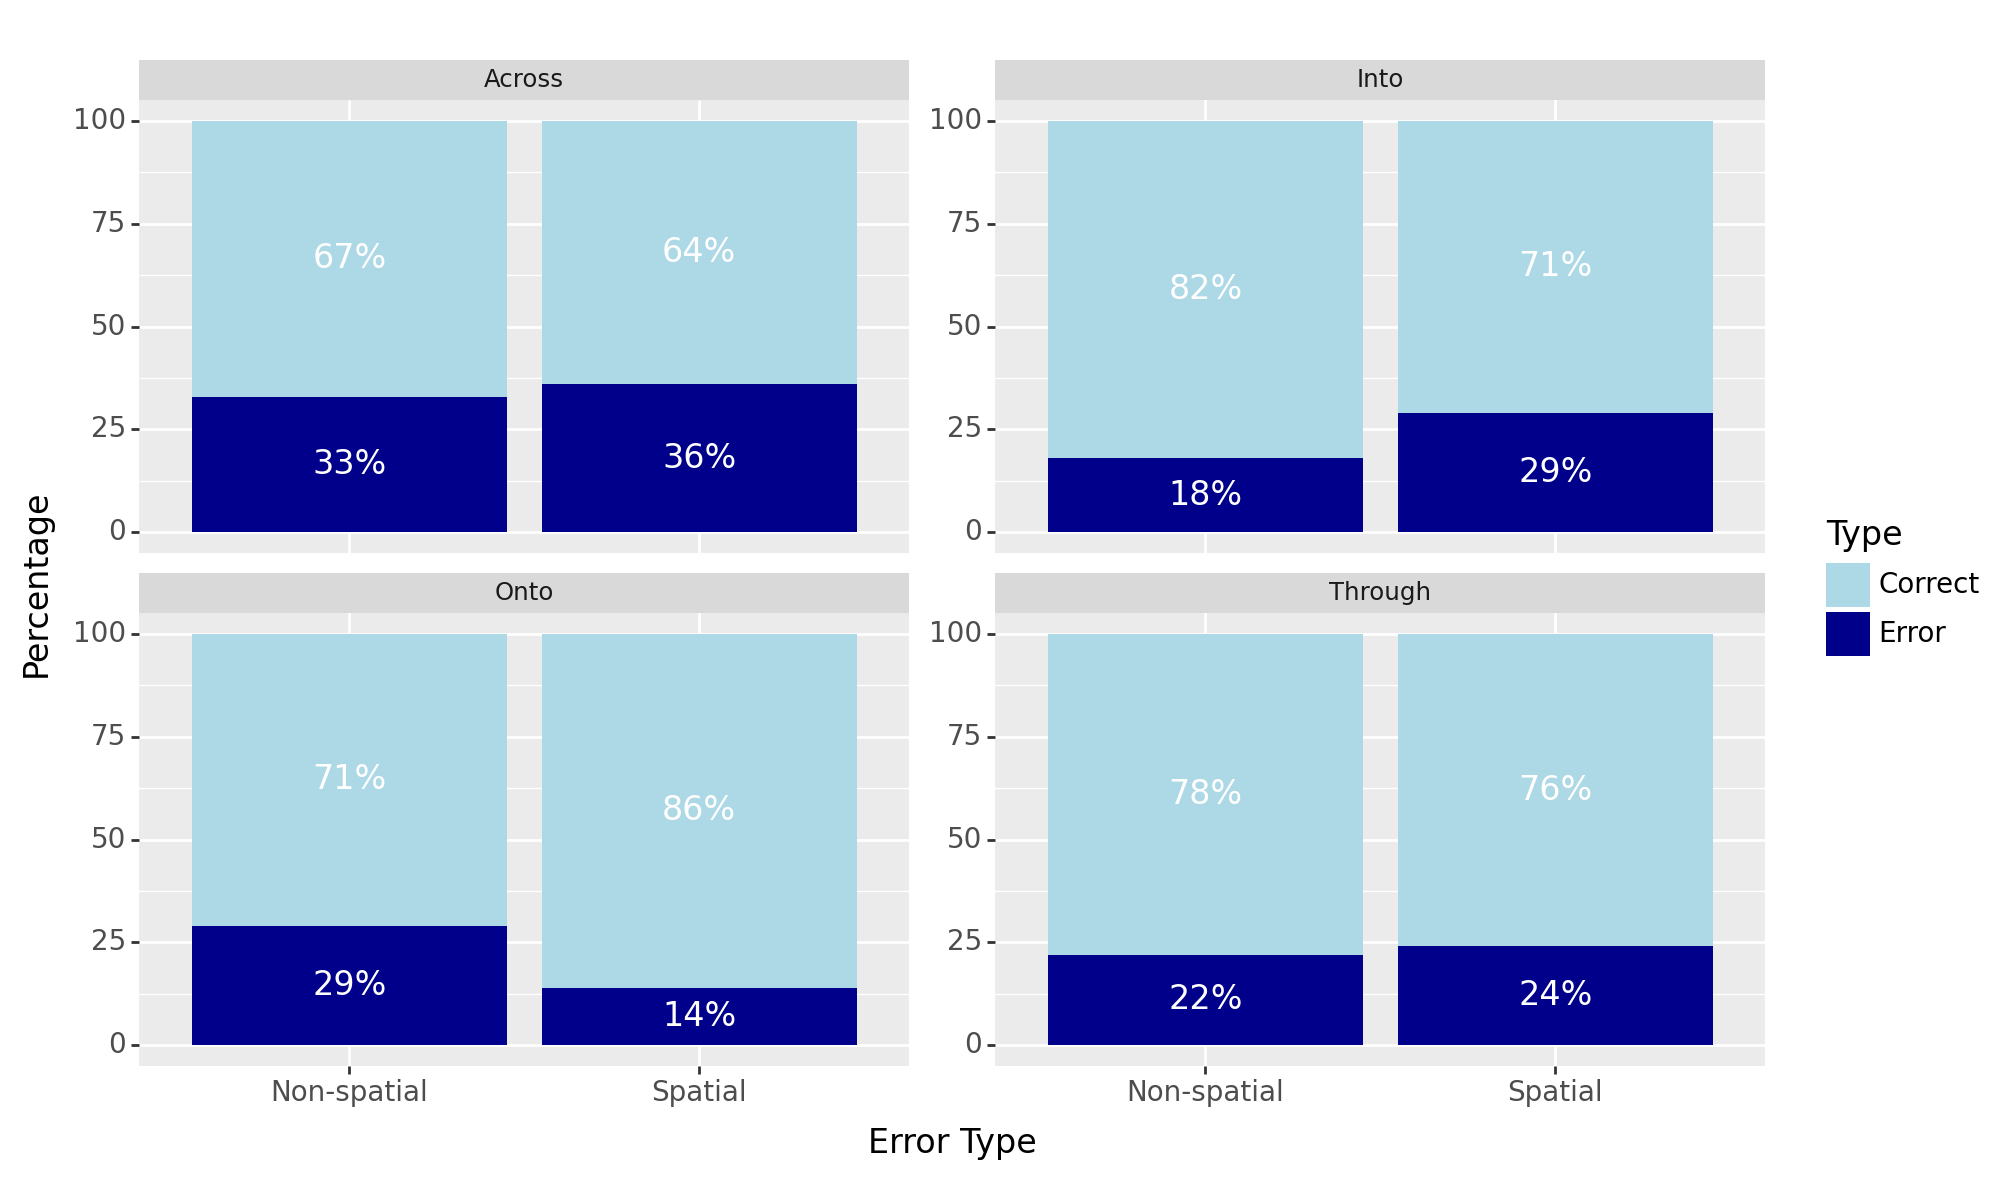
\includegraphics[width=1\textwidth]{textual/Figuras/Results/Unknown-52.png}
        \caption{Spatial vs. Non-spatial: Correct Translations and Errors by Preposition (\%).}
        \label{fig: spatial-non-perc}
\end{figure}

%We observed significant disparities in error types across preposition pairs. For instance, ACROSS was the only preposition that had considerably fewer non-spatial errors ($7$ instances, $21.9\%$ of total) but predominant spatial errors ($25$ out of $32$ instances, $78.1\%$) (See Example~\ref{ex:ex-12} for an illustration of spatial error with ACROSS). Conversely, THROUGH showcased noticeable high non-spatial errors ($73$ instances, approximately $69.5\%$ of total) and lower than half that number in spatial errors ($32$ instances, about $30.5\%$). Similarly, INTO had more prevalent non-spatial errors ($112$ instances, approximately $67.1\%$ of total) compared to spatial errors ($55$ instances, about $32.9\%$). Also, ONTO exhibited dominant non-spatial errors ($8$ instances, approximately $72.7\%$ of total) and fewer spatial errors ($3$ instances, roughly $27.3\%$) (See Example~\ref{ex:ex-13} for an illustration of non-spatial error with ONTO). 

\subsubsection{ACROSS} 

In this subsection, we analyze the occurrence count, correct count, error count, correct rate, and error rate for the preposition ACROSS, divided into non-spatial and spatial categories. The detailed statistics are presented in Table~\ref{tab:across}. The analysis reveals that, for ACROSS, the spatial category outperformed the non-spatial category in nearly all metrics: $70$ occurences vs. $21$, $45$ correct translations vs. $14$, and $25$ errors vs. $7$, with the exception of a marginal two-point difference in correct proportion ($64.28\%$ vs. $66.66\%$). Although the error rate is slightly higher for spatial ($\approx36\%$) compared to non-spatial ($\approx33\%$), we can safely affirm both categories exhibit a similar trend. This indicates that, for ACROSS, spatial and non-spatial errors may present comparable levels of difficulty, despite the first group's higher frequency. Overall, for ACROSS, spatial senses may be only slightly more prone to errors than non-spatial senses. Example~\ref{ex:ex-12} illustrates a case of spatial error with ACROSS.


\begin{table}[htb]
\centering
\begin{tabular}{lcc}
\toprule
 & \multicolumn{2}{c}{\textbf{ACROSS}} \\ 
 & \textbf{N-SP} & \textbf{SP} \\ 
\midrule
Ocurrence Count & $21$ & $70$ \\ 
Correct Count & $14$ & $45$ \\ 
Error Count & $7$ & $25$ \\ 
\midrule
Correct Rate & $\mathbf{66.66\%}$ & $64.28\%$ \\ 
\midrule
Error Rate & $33.33\%$ & $\mathbf{35.71\%}$ \\ 
\bottomrule
\end{tabular}
\caption{ACROSS: Spatial (SP) vs. Non-Spatial (N-SP): Counts and Rates.}
\label{tab:across}
\end{table}


\ex.\texttt{(inner\_id: 27316)} \hfill \texttt{Across(ii)} \\[0.3ex]
\noindent\rule{\linewidth}{0.9pt}
When I \colorbox{lightblue}{\textcolor{blue}{walked}} \colorbox{lightgray}{\textcolor{blue}{\emph{across}}} \colorbox{lightgray}{\textcolor{blue}{Afghanistan}}, I \textcolor{blue}{stayed} with people like this. (SRC) \label{ex:ex-12} \\[-0.3ex]
\noindent\rule{\linewidth}{0.3pt}
Quando \colorbox{lightgray}{\textcolor{ForestGreen}{\emph{atravessei}}} \colorbox{lightgray}{\textcolor{ForestGreen}{o Afeganistão}} \colorbox{lightblue}{\textcolor{ForestGreen}{a pé}}, \textcolor{ForestGreen}{fiquei} em casas de pessoas como esta. (REF) \\[-0.3ex]
\noindent\rule{\linewidth}{0.3pt}
?~Quando \colorbox{lightgray}{\textcolor{Maroon}{\emph{passei pela}}} \colorbox{lightgray}{\textcolor{Maroon}{Áfgão}}, \textcolor{Maroon}{passei} com pessoas como essas. (Gemma-7B) \\[-0.3ex]
\noindent\rule{\linewidth}{0.9pt}

In Example~\ref{ex:ex-12}, a spatial error involving syntactic projection (sp) is observed in the use of the preposition ACROSS. Here, the phrase ``passei pela'' incorrectly attempts to translate the spatial expression by adopting the EN lexicalization pattern of expressing motion into PT-br, a practice deemed incorrect by the literature \parencite{talmy2000towardb, slobin2005relating, McCleary-Viotti-2004}. Although the Manner element in ``walked'' is not directly translated in ``passei'' (passed), we considered this error a syntatic projection because it reflects an attempt at directly translating the EN construction. It is also worth noting that we consider the expression ``passar pelo(a) more closer in meaning with ``(go) through'' than with ``across''. Additionally, ``pela'' constitutes an agreement (ag) error, ``Áfgão'' an interlanguage/code-switching (in) error, and ``passei'' a wrong lexical choice (wl) error.


\subsubsection{$\chi^2$ Test Results for ACROSS} 

Following the analysis, the Chi-Square ($\chi^2$) Test was conducted to determine if there was a significant association between the number of errors (spatial vs. non-spatial) and correct instances in the translations. For ACROSS, the test yielded a chi-square statistic of $0.0$ (threshold is  $\chi^2 > 3.841$), a p-value of $1.0$ (threshold is  $p < 0.05$), and $1$ degree of freedom (df), indicating that the observed frequencies are very close to the expected frequencies. This result suggests no significant association between the two categories, meaning that, for this preposition, spatial and non-spatial errors do not differ significantly in their impact on overall translation accuracy. The high p-value implies that the observed distribution is entirely consistent with the null hypothesis of independence between the categories. The graph in Figure~\ref{fig: schi-across} illustrates the expected vs. observed values, highlighting this consistency and showing only slight differences such as in lower observed values in some categories.

\begin{figure}[htb]
        \centering
        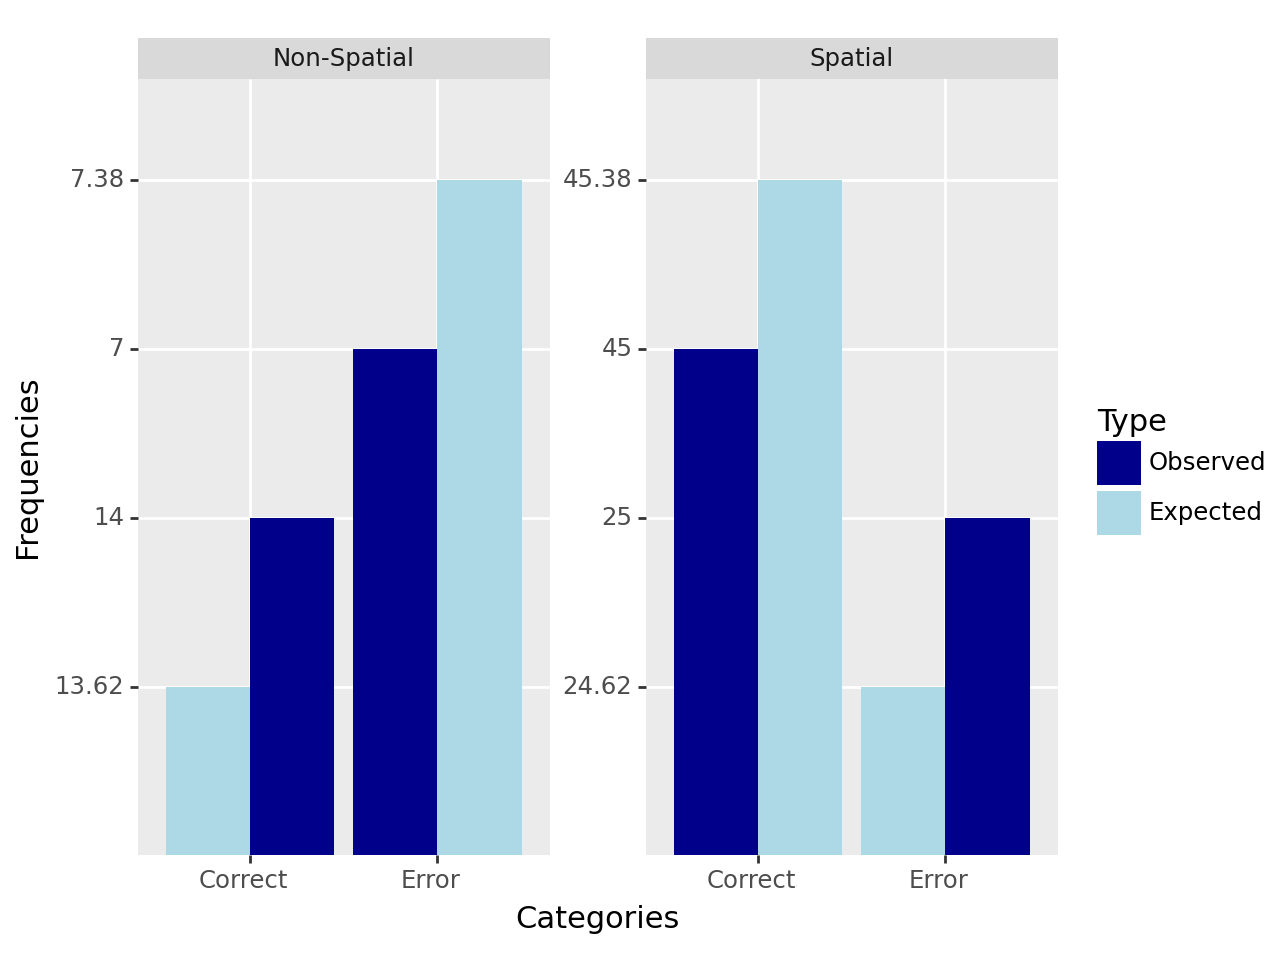
\includegraphics[width=.8\textwidth]{textual/Figuras/Results/Unknown-65.png}
        \caption{ACROSS: Observed vs. Expected Frequencies.}
        \label{fig: schi-across}
\end{figure}


\subsubsection{INTO} 

In this subsection, we provide an overview of the results for INTO. Table~\ref{tab:into} summarizes the occurrence count, correct count, error count, correct rate, and error rate obtained for INTO by category: spatial and non-spatial. The analysis reveals an interesting pattern across the statistics for the preposition INTO. While the non-spatial category presented significantly higher numbers in almost all metrics: occurrence count ($609$ vs. $189$), correct count ($497$ vs. $134$), error count ($112$ vs. $55$), and correct rate ($\approx82\%$ vs. $\approx71\%$), interestingly, its error rate was actually considerably lower ($\approx18\%$) compared to the spatial category ($\approx29\%$). This finding suggests that, while non-spatial senses were considerably more frequent for INTO, spatial senses were significantly more prone to errors, with an 11-point margin.


\begin{table}[htb]
\centering
\begin{tabular}{@{}lccc@{}} \\
\toprule
& \multicolumn{2}{c}{\textbf{INTO}} \\ 
& \textbf{N-SP} & \textbf{SP} \\
\midrule
Occurrences & $609$ & $189$\\
Correct Count  & $497$ & $134$\\
Error Count & $112$ & $55$ \\
\midrule
Correct Rate & $\mathbf{81.60\%}$ & $70.89\%$\\
\midrule
Error Rate & $18.39\%$ & $\mathbf{29.10\%}$\\
\bottomrule
\end{tabular}
\caption{INTO: Spatial (SP) vs. Non-Spatial (N-SP): Counts and Rates.} \label{tab:into} 
\end{table}


\subsubsection{$\chi^2$ Test Results for INTO} 

The analysis of the Chi-Square ($\chi^2$) Test for INTO further confirms the previous results, yielding a chi-square statistic of $9.361$ (threshold is  $\chi^2 > 3.841$), a p-value of $0.0022$ (threshold is $p < 0.05$), and $1$ degree of freedom (df). These results suggest a significant correlation between the number of errors (spatial vs. non-spatial) in translations for this preposition, rejecting the null hypothesis. This indicates that the spatial and non-spatial errors in translations for INTO are not independent and are likely influenced by some underlying factor. As can be seen in Figure~\ref{fig: schi-into}, observed frequencies deviate significantly (more than 10 points) from what would be expected if there were no association between these categories, emphasizing the strength of this correlation.

\begin{figure}[htb]
        \centering
        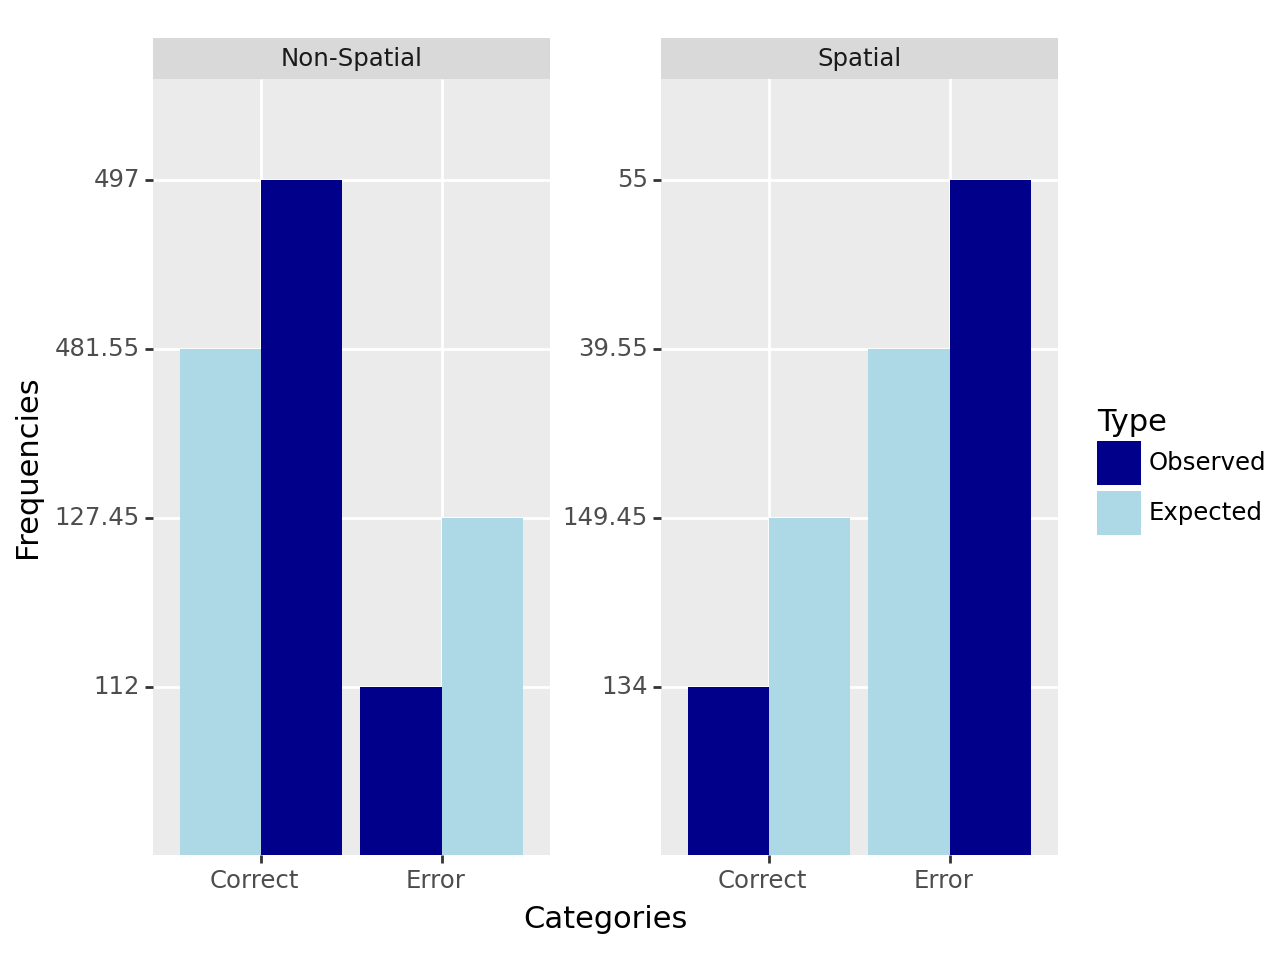
\includegraphics[width=.8\textwidth]{textual/Figuras/Results/Unknown-66.png}
        \caption{INTO: Observed vs. Expected Frequencies.}
        \label{fig: schi-into}
\end{figure}


\subsubsection{ONTO}

In this subsection, we present the results for ONTO. Table~\ref{tab:onto} displays the occurrence count, correct count, error count, correct rate, and error rate for ONTO categorized as spatial and non-spatial. The analysis reveals that non-spatial senses were slightly higher in nearly all metrics, except for error rate (with $\approx29\%$ for non-spatial compared to $\approx14\%$ for spatial senses). This second group exhibited only slightly fewer errors ($3$) compared to the first ($8$). This trend persisted across the occurrence count ($21$ vs. $28$) and correct count ($3$ vs. $8$), resulting in a lower error rate for spatial senses ($\approx14\%$) compared to non-spatial senses ($\approx29\%$). These findings suggest that non-spatial errors were marginally more frequent and presented a significantly bigger challenge than spatial errors. Example~\ref{ex:ex-13} illustrates a case with ONTO.

\begin{table}[htb]
\centering
\begin{tabular}{@{}lccc@{}} \\
\toprule
& \multicolumn{2}{c}{\textbf{ONTO}} \\ 
& \textbf{N-SP} & \textbf{SP} \\
\midrule
Occurrences & $28$ & $21$ \\
Correct Count & $20$ & $18$ \\
Error Count & $8$ & $3$ \\
\midrule
Correct Rate & $71.42\%$ & $\mathbf{85.71\%}$ \\
\midrule
Error Rate & $\mathbf{28.57\%}$ & $14.29\%$ \\
\bottomrule
\end{tabular}
\caption{ONTO: Spatial (SP) vs. Non-Spatial (N-SP) Counts and Rates.} \label{tab:onto} 
\end{table}


\ex.\texttt{(inner\_id: 32495)} \hfill \texttt{Onto(iii)} \\[0.3ex]
\noindent\rule{\linewidth}{0.9pt}
And the business organizations thought we \colorbox{lightgray}{\textcolor{blue}{were \emph{onto} something}} in terms of a way of preparing children much better for \textcolor{blue}{real-life work} today. (SRC) \label{ex:ex-13} \\[-0.3ex]
\noindent\rule{\linewidth}{0.3pt}
E as organizações empresariais acharam que \colorbox{lightgray}{\textcolor{ForestGreen}{tínhamos algo interessante}} em termos de um preparo muito melhor das crianças para \textcolor{ForestGreen}{trabalhos da vida real} dos dias de hoje. (REF) \\[-0.3ex]
\noindent\rule{\linewidth}{0.3pt}
?~E as organizações empresariais acharam que \colorbox{lightgray}{\textcolor{Maroon}{estávamos \emph{em} algo}} quando se tratava de preparar muito melhor as crianças para \textcolor{Maroon}{o trabalho real da vida} hoje. (Mixtral-8x7B) \\[-0.3ex]
\noindent\rule{\linewidth}{0.9pt}

Example~\ref{ex:ex-13} contains a case of non-spatial error involving an idiomatic expression (ie) with the preposition ONTO.  In this instance, the PT-br phrase ``estávamos em algo'' can be considered an overly-literal translation of the idiom ``(be) onto something,'' which in this context means ``having done or discovered something important, special, etc.'' according to the \textcite{merriamwebster_onto_something} dictionary. One possible way of expressing this idea in PT-br is ``tínhamos algo interessante,'' such as in the reference (REF). Furthermore, ``o trabalho REAL da vida'' constitutes an interesting case of grammar/orthography (gr) error involving incorrect word order, which, in this case, completely changed the original meaning of ``trabalho da vida REAL'' (real-life work).


\subsubsection{$\chi^2$ Test Results for ONTO} 

The analysis of the Chi-Square ($\chi^2$) Test for ONTO yielded a chi-square statistic of $0.706$ (threshold is  $\chi^2 > 3.841$), a p-value of $0.401$ (threshold is  $p < 0.05$), and $1$ degree of freedom (df). These results indicate that there is no significant correlation between the number of errors (spatial vs. non-spatial) in translations for the ONTO preposition, as the p-value exceeds the typical significance level of $0.05$. The expected frequencies, as illustrated in Figure~\ref{fig: schi-onto}, further support this conclusion, with observed frequencies closely aligning (less than 2 points) with what would be expected under the null hypothesis of independence between the categories.

\begin{figure}[htb]
        \centering
        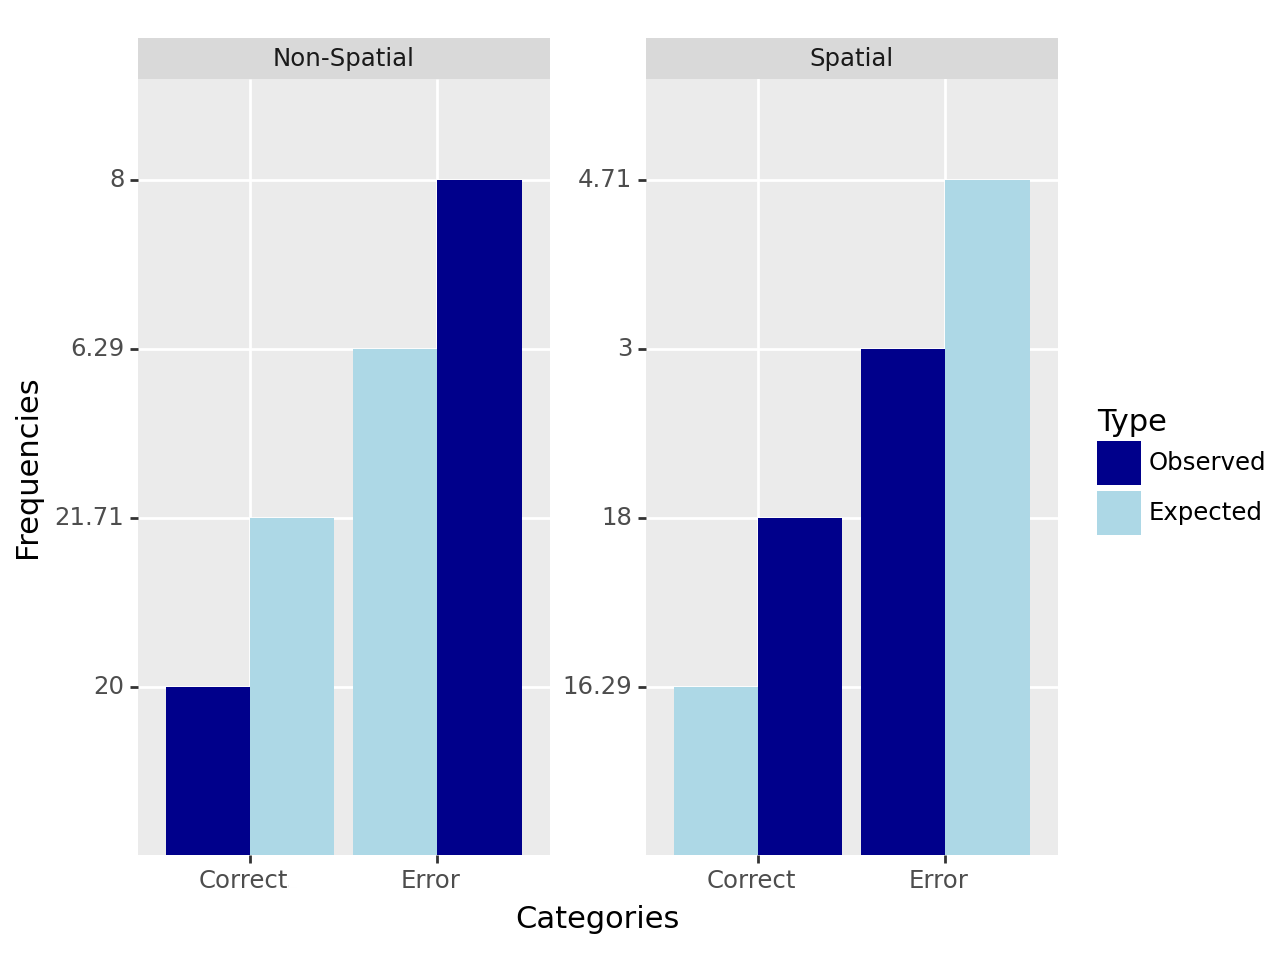
\includegraphics[width=.8\textwidth]{textual/Figuras/Results/Unknown-67.png}
        \caption{ONTO: Observed vs. Expected Frequencies.}
        \label{fig: schi-onto}
\end{figure}


\subsubsection{THROUGH}

Table~\ref{tab:through} provides a summary of the occurrences, correct count, error count, correct rate, and error rate associated with the preposition THROUGH, categorized as spatial and non-spatial. The analysis indicates that non-spatial senses exhibited a considerably higher number of occurrences ($336$) compared to spatial senses ($133$), as well as correct count ($263$ vs. $101$), error count ($73$ vs. $32$), resulting in a slightly higher correct rate ($\approx79\%$ vs. $\approx76\%$). However, despite these higher numbers, we observe a slightly lower error rate for this category ($\approx22\%$) compared to spatial senses ($\approx24\%$). This suggests that, while non-spatial senses were more prevalent, spatial senses had a slightly higher error proportion, indicating an almost comparable challenge in their accurate usage.

\begin{table}[htb]
\centering
\begin{tabular}{@{}lccc@{}} \\
\toprule
& \multicolumn{2}{c}{\textbf{THROUGH}} \\ 
& \textbf{SP} & \textbf{N-SP} \\
Occurrences & $133$ & $336$ \\
Correct Count & $101$  & $263$\\
Error Count & $32$ & $73$ \\
\midrule
Correct Rate & $75.93\%$ & $\mathbf{78.72\%}$ \\
\midrule
Error Rate & $\mathbf{24.06\%}$ & $21.73\%$ \\
\bottomrule
\end{tabular}
\caption{THROUGH: Spatial (SP) vs. Non-spatial (N-SP) Counts and Rates.} \label{tab:through} 
\end{table}

\subsubsection{$\chi^2$ Test Results for THROUGH} 

The Chi-Square ($\chi^2$) Test conducted for the preposition THROUGH resulted in a chi-square statistic of $0.179$ (threshold is $\chi^2 > 3.841$), with a corresponding p-value of $0.672$ (threshold is $p < 0.05$) and $1$ degree of freedom (df). These findings suggest that there is no significant correlation between the number of errors (spatial vs. non-spatial) in translations for this preposition, as the p-value far exceeds the conventional significance level of $0.05$. Moreover, as illustrated in Figure~\ref{fig: through-chi}, the observed frequencies closely match the expected frequencies (with less than 3 points) under the assumption of independence between the categories. Thus, the data does not provide sufficient evidence to reject the null hypothesis of independence.

\begin{figure}[htb]
        \centering
        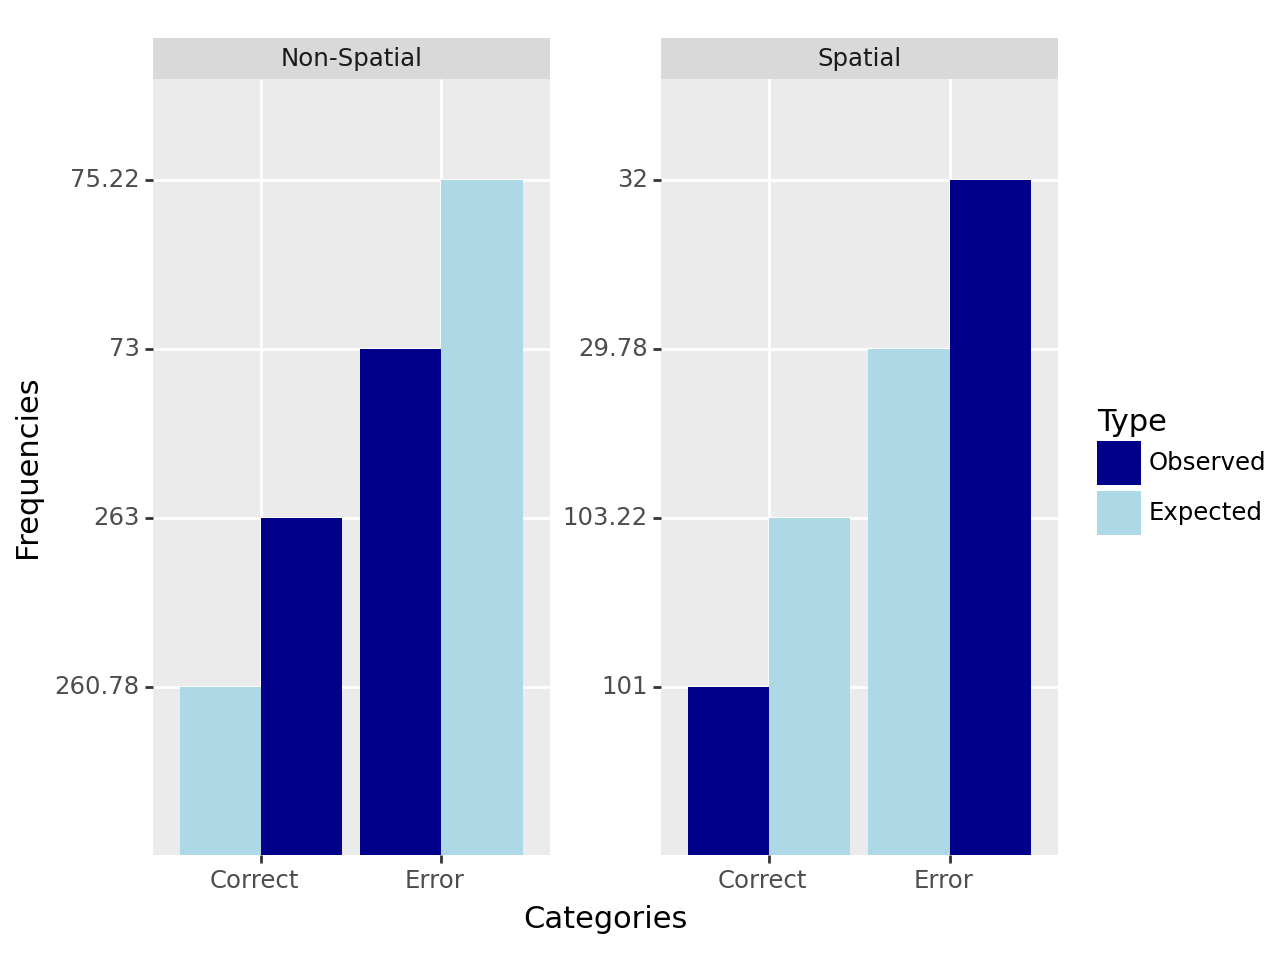
\includegraphics[width=.7\textwidth]{textual/Figuras/Results/Unknown-68.png}
        \caption{THROUGH: Observed vs. Expected Frequencies.}
        \label{fig: through-chi}
\end{figure}


%Based on our findings, we hypothesize whether the frequency of a given preposition in real-world scenarios could potentially impact the errors observed in our analysis. We noted that spatial errors were more common for prepositions that are less frequent in idioms and phrasal verbs, such as ACROSS. This suggests that, in this case, translating spatial relationships may pose greater challenges. Conversely, we observed significant variation in non-spatial error prevalence for INTO, indicating that there may be nuanced difficulties in translating idiomatic expressions. One potential explanation, we thought, might be the higher occurrence of phrasal verbs and idioms containing INTO compared to ACROSS, which could contribute to models' struggles with non-spatial errors.

%To confirm our premise, we compiled a list of phrasal verbs from \texttt{Wiktionary}\footnote{\href{https://en.wiktionary.org/wiki/Wiktionary:Main\_Page}{https://en.wiktionary.org/wiki/Wiktionary:Main\_Page}} by Wikipedia using JSON data and then filtered them by preposition to ascertain their incidence for each of the four prepositions we analyzed. The results are summarized in Table~\ref{tab:prevalence}. For the complete lists of phrasal verbs, please refer to the Attachments Section (Tables~\ref{a:across} (for ACROSS), \ref{a:into} (for INTO), \ref{a:onto} (for ONTO), \ref{a:through} (for THROUGH)).

%\begin{table}[ht]
%\centering
%\begin{tabular}{@{}lcc@{}} \\
%\midrule
%\toprule
%\textbf{Preposition} & \textbf{N. of Phrasal Verbs} \\
%\midrule
%Across  & $11$ \\
%Into & \colorbox{lightgray}{$61$} \\
%%%%Onto & $11$ \\
%%%Through & \colorbox{lightgray}{$60$} \\
%%\bottomrule
%\midrule
%\end{tabular}
%\caption{Prevalence of Prepositions in Phrasal Verbs (Source: Wiktionary by Wikipedia).} \label{tab:prevalence} 
%\end{table}

%These findings confirm that the prevalence of spatial prepositions in EN phrasal verbs varies considerably. We observed a potential correlation between the frequency of phrasal verbs and the distribution of non-spatial errors. For instance, prepositions like INTO and THROUGH, which have more phrasal verbs, showed a greater prevalence of non-spatial errors, indicating that their complexity may affect the models' performance. On the other hand, the lower occurrence of ONTO phrasal verbs may explain its relatively lower non-spatial counts, and, possibly, its low spatial error rate. Overall, this analysis suggests that ACROSS and ONTO may be less frequently used in real-world spatial descriptions, and since the realm of idiomatic expressions is an extension of the spatial domain, as described by Cogitive Theorists like ~\textcite{LakoffJohnson80, coventry:04b}, this could make them less common in non-spatial description as well.

%Overall, these insights highlight the complexity of EN idiomatic expression usage and its impact on NMT. Understanding the relationship between the use of spatial prepositions in phrasal verbs and error distribution can guide the development of targeted strategies to enhance the quality of NMT systems.

\subsection{Analysis by Meaning: Spatial vs. Non Spatial Errors}
\label{subsec: sp-vs-nsp}

This analysis extends the previous investigation. Our main goal was to identify which specific meanings associated with each preposition (please refer back to Table~\ref{tab:prep-categorizations} for the complete list) most adversely impacted the translations. We were particularly interested in discovering which spatial meanings of ACROSS, THROUGH, INTO, and ONTO, as defined by \textcite{bruckfield2011prepositions}, significantly influenced the quality of the translations.

We used the same two distinct groups of errors from the previous analysis: ``Spatial,'' consisting of polysemy (po), syntactic projection (sp), and wrong sense (ws) errors, and ``Non-spatial,'' consisting of idiomatic expression (ie) errors. Figure~\ref{fig: all-perc} offers an overview of the distribution of correct translations and errors for each preposition by meaning. Table~\ref{tab:combined}, in Attachment~\ref{att2}, provides an overview of the occurrence count, correct count, error count, correct rate, and error rate for the two groups.

\begin{figure}[htb]
        \centering
        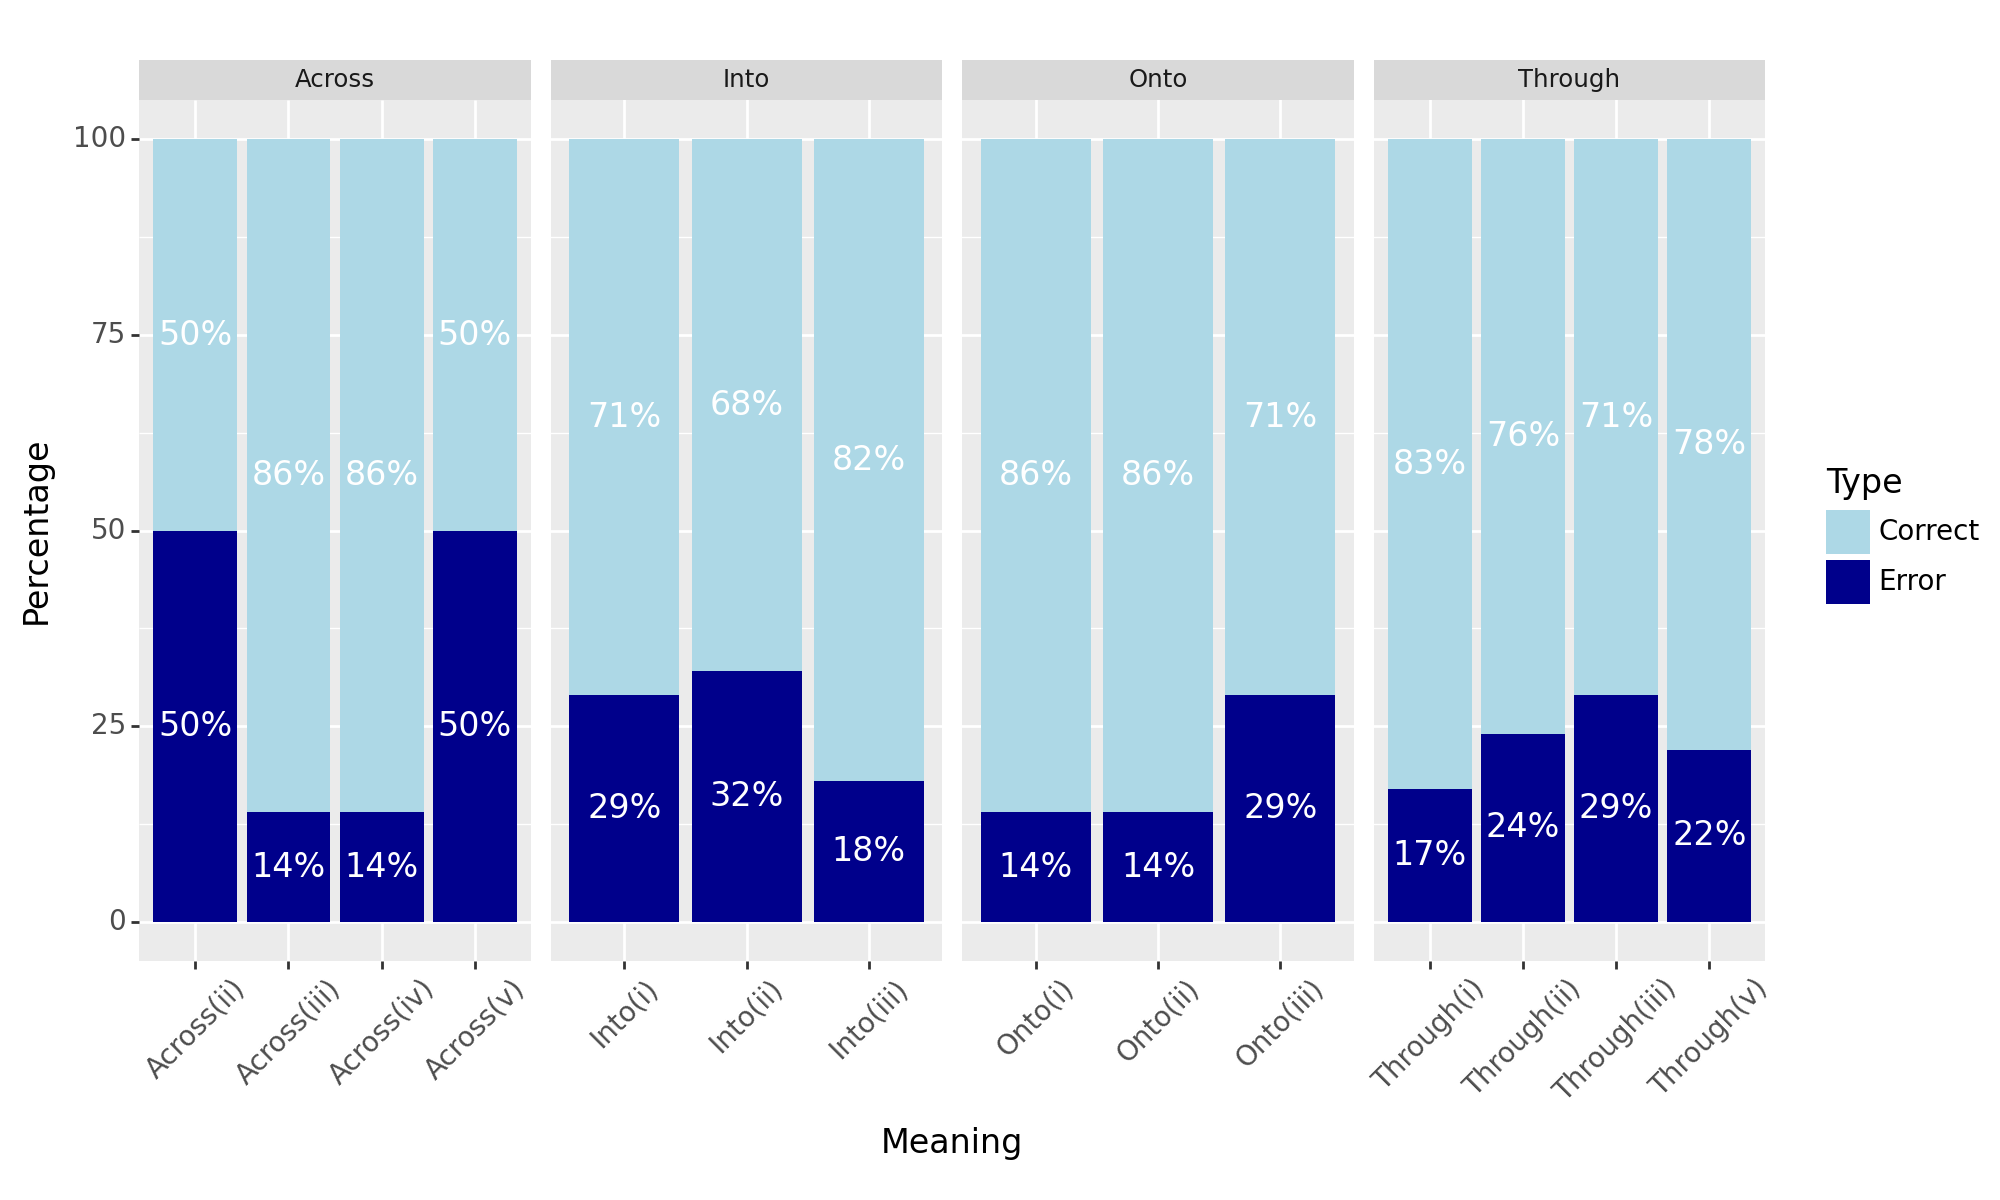
\includegraphics[width=1\textwidth]{textual/Figuras/Results/Unknown-71.png}
        \caption{ACROSS, INTO, ONTO, and THROUGH: Correct and Error Rates by Meaning (\%).}
        \label{fig: all-perc}
\end{figure}

\subsubsection{ACROSS by Meaning}

In this subsection, we present the number of occurrences, correct count, error count, correct rate, and error rate for ACROSS by meaning. Table~\ref{tab:across-senses} displays these statistics. 

The results reveal significant variations in the performance of models across different meanings of ACROSS. For spatial meanings, both ``Across(iii) -- Opposite location'' and ``Across(iv) -- Distribution'' exhibit the highest correct proportions, each at $\approx86\%$. Conversely, the non-spatial meaning ``Across(v)'' and ``Across(ii) -- Movement over a surface'' show lower correct rates, both at $50\%$. Notably, the error rates mirror this trend, with ``Across(ii)'' and ``Across(v)'' having the highest error rates at $50\%$, indicating these meanings presented more challenges for accurate translation. These rates underscore the models' strengths in handling specific spatial contexts while highlighting the need for improvement in non-spatial and ``Across(ii)'' contexts.


\begin{table}[htb]
\centering
\begin{tabular}{lcccc}
\toprule
 & \multicolumn{4}{c}{\textbf{ACROSS by Meaning}} \\ 
 & \multicolumn{3}{c}{\textbf{SP}} & \textbf{N-SP} \\ 
 & Across(ii) & Across(iii) & Across(iv) & Across(v) \\
\midrule
Occurrences & $42$ & $7$ & $21$ & $14$ \\
Correct Count & $21$ & $6$ & $18$ & $7$ \\ 
Error Count & $21$ & $1$ & $3$ & $7$ \\ 
\midrule
Correct Rate & $50.00\%$ & $\mathbf{85.71\%}$ & $\mathbf{85.71\%}$ & $50.00\%$ \\ 
\midrule
Error Rate & $\mathbf{50.00\%}$ & $14.28\%$ & $14.28\%$ & $\mathbf{50.00\%}$ \\ 
\bottomrule
\end{tabular}
\caption{ACROSS: Spatial (SP) vs. Non-spatial (N-SP) Counts and Rates by Meaning.}
\label{tab:across-senses}
\end{table}


\subsubsection{$\chi^2$ Test Results for ACROSS by Meaning} 

The Chi-square analysis of the data from Table~\ref{tab:across-senses} reveals a Chi-square statistic of $10.10$  (threshold is $\chi^2 > 7.815$) with a p-value of $0.018$ (threshold is $p < 0.05$) and $3$ degrees of freedom (df) of. The difference between expected and observed frequencies for the correct and error counts across the different meanings of ACROSS are illustrated in Figure~\ref{fig:across-senses-chi}. The p-value of $0.018$, being less than the typical significance level of $0.05$, indicates that there is a statistically significant difference in the distribution of correct and error counts across the different meanings of ACROSS. This suggests that the models do not perform equally across all meanings, highlighting specific areas where the models struggle, particularly with the non-spatial meaning and the "Movement over a surface" meaning. This underscores the necessity for further refinement in handling these contexts.

\begin{figure}[htb]
        \centering
        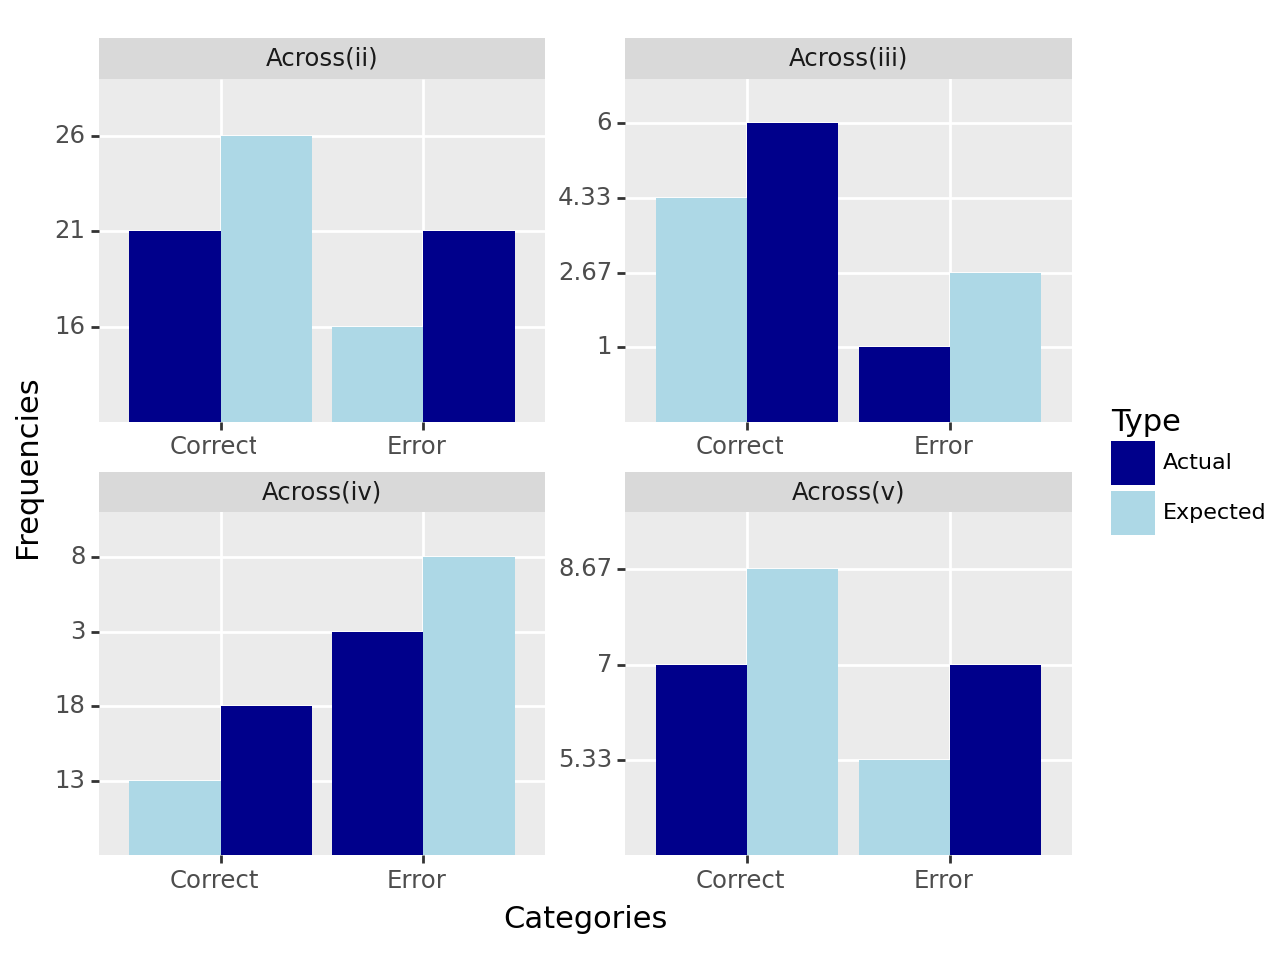
\includegraphics[width=.8\textwidth]{textual/Figuras/Results/Unknown-70.png}
        \caption{ACROSS: Observed vs. Expected Frequencies by Meaning.}
        \label{fig:across-senses-chi}
\end{figure}


%Once again, we observed significant disparities in the occurrences of errors caused by the different preposition senses. For instance, out of the $25$ spatial errors identified for ACROSS, $21$ are associated with the sense Across(2), which indicates ``movement over a surface'', " comprising a surprising $65\%$ of instances. The second largest group was Across(5), which is when the preposition is ``non-spatial'', with $21.9\%$ ($7$ errors). The remaining spatial senses, Across(4), ``distribution'' and Across(3), ``opposite location'', together comprise $12.5\%$ (with $4$ errors in total). Conversely, for INTO, the sense Into(1) ``movement leading to enclosure'' had the highest number of spatial errors, with $46$ ($27.5\%$), followed by Into(2), which indicates ``movement resulting in collision,'' with $9$ errors ($5.4\%$). The highest proportion of errors ($67\%$) was still observed in the sense Into(3), denoting ``non-spatial'' use, with a massive $112$ errors. THROUGH had similar behavior, with the majority of errors ($73$, or $69.5\%$) connected to the ``non-spatial'' sense THROUGH(5). Out of the $32$ spatial errors, $19.0\%$ are connected to sense THROUGH(3) ``movement past a barrier,'' $6.7\%$ are connected to ``movement within a passage/conduit'', THROUGH (1), and $4.8\%$ are connected to ``movement within an open area'', THROUGH(2), with $20$, $7$, and $5$ errors, respectively. And lastly, ONTO, which showed the smallest number of occurences, had $8$ ``non-spatial'' errors (sense ONTO(3)) and a total of $3$ spatial erros, with senses ONTO(1), ``movement to a surface'', comprising $18.2\%$ and ONTO(2), ``sense of attachment'', comprising $9.1\%$ \parencite{bruckfield2011prepositions, cambridge-across, cambridge-into, cambridge-onto, cambridge-through}. For your information, senses ACROSS(1), ``perpendicular position'' and THROUGH(4), ``part of a route'' were not identified in the sample for human review.

\subsubsection{INTO by Meaning}

This subsection presents the number of occurrences, correct count, error count, correct rate, and error rate for each meaning of INTO. Table~\ref{tab:into-senses} displays this statistics.  The results illustrate varying performance across different senses of INTO. The non-spatial meaning ``Into(iii)'' shows the highest correct rate at $\approx82\%$, indicating strong translation capabilities. Conversely, spatial meanings ``Into(i)'' and ``Into(ii)'' exhibit slightly lower correct proportions at $\approx71\%$ and $\approx68\%$, respectively. Error proportions reveal challenges in translating spatial meanings, with ``Into(ii)'' showing the highest error rate at $\approx32\%$. In contrast, the non-spatial meaning ``Into(iii)'' has a lower error rate at $\approx18\%$, suggesting better performance. These findings underscore the models' varying proficiency across different senses of INTO, with potential implications for improving translation accuracy, particularly in spatial contexts such as ``Movement or direction leading to enclosure'' and ``Movement resulting in physical contact or collision.''


\begin{table}[htb]
\centering
\begin{tabular}{lccc}
\toprule
 & \multicolumn{3}{c}{\textbf{INTO by Meaning}} \\ 
 & \multicolumn{2}{c}{\textbf{SP}} & \textbf{N-SP} \\ 
 & Into(i) & Into(ii) & Into(iii) \\
\midrule
Occurrences & $161$ & $28$ & $609$ \\ 
Correct Count & $115$ & $19$ & $497$ \\ 
Error Count & $46$ & $9$ & $112$ \\ 
\midrule
Correct Rate & $\mathbf{71.42\%}$ & $67.85\%$ & $\mathbf{81.60\%}$ \\
\midrule
Error Rate & $28.57\%$ & $\mathbf{32.14\%}$ & $18.39\%$
\\ 
\bottomrule
\end{tabular}
\caption{INTO: Spatial (SP) vs. Non-Spatial (N-SP) Counts and Rates by Meaning.}
\label{tab:into-senses}
\end{table}


\subsubsection{$\chi^2$ Test Results for INTO by Meaning} 

The Chi-square examination of the data from Table~\ref{tab:into-senses} resulted in a Chi-square value of $10.18$ (threshold is $\chi^2 > 5.991$), accompanied by a p-value of $0.006$ (threshold is $p < 0.05$) and degrees of freedom (df) of $2$. The disparity between expected and observed frequencies across the distinct meanings of INTO is depicted in Figure~\ref{fig: into-mean-chi}. With a p-value of $0.006$, notably lower than the standard significance level of $0.05$, the analysis underscores a statistically notable distinction in the distribution of accurate and erroneous counts among the various interpretations of INTO. This disparity suggests divergent performance among models across these interpretations, pinpointing specific domains that may benefit from refinement, particularly in spatial translation contexts.

\begin{figure}[htb]
        \centering
        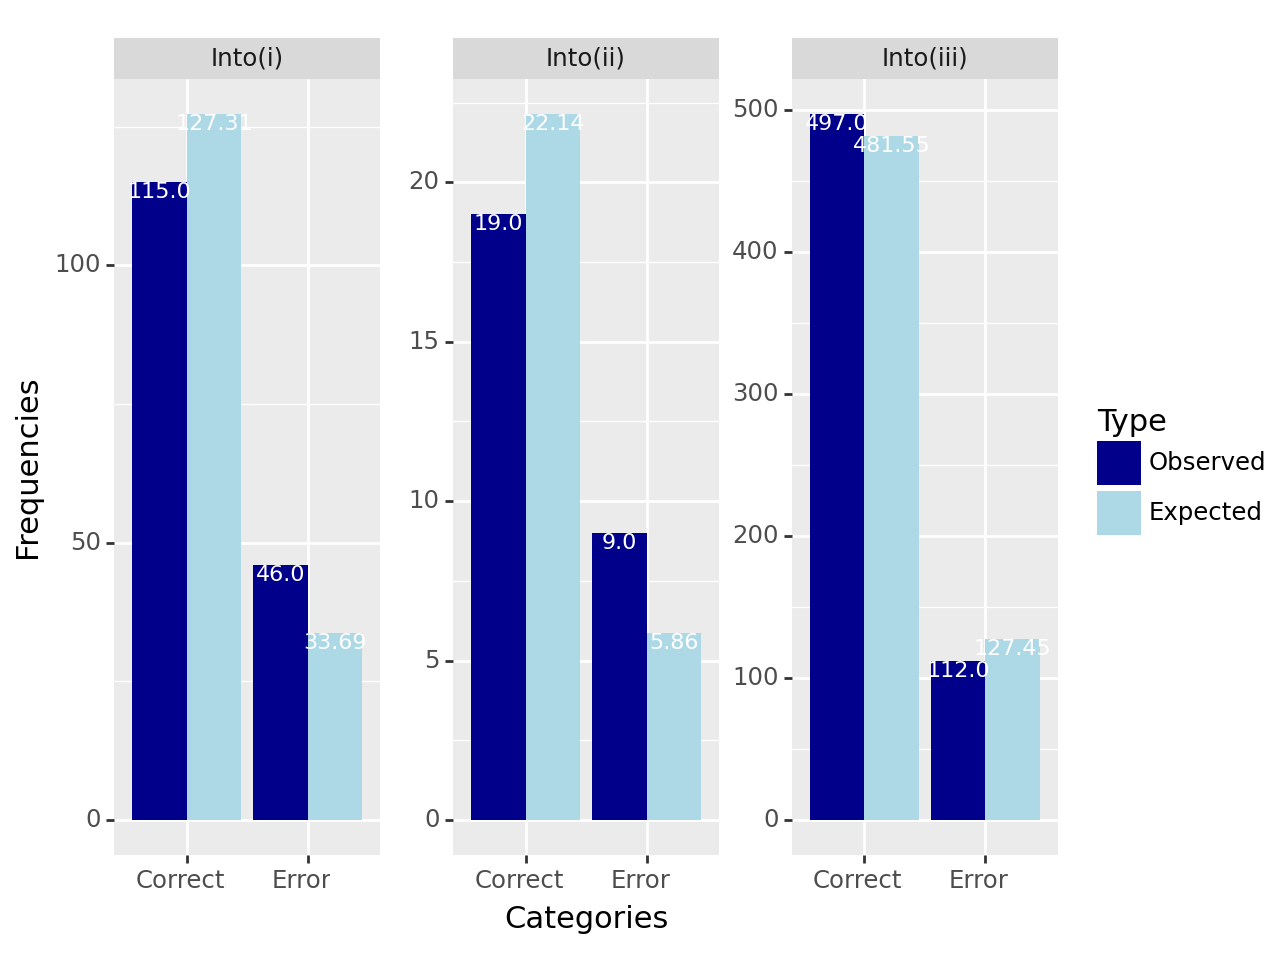
\includegraphics[width=.8\textwidth]{textual/Figuras/Results/Unknown-81.png}
        \caption{INTO: Observed vs. Expected Frequencies by Meaning (\%).}
        \label{fig: into-mean-chi}
\end{figure}

\subsubsection{ONTO by Meaning}

Table~\ref{tab:onto-mean} presents an analysis of translation performance across different meanings of ONTO. In spatial contexts, both ``Onto(i) -- Movement to a location on a surface'' and ``Onto(ii) -- Sense of attachment'' exhibit high correct rates, each at $\approx86\%$. This indicates strong translation accuracy for these spatial meanings. Conversely, the non-spatial meaning ``Onto(iii)'' demonstrates a lower correct proportion at $\approx71\%$, suggesting comparatively more challenges in accurately translating non-spatial contexts. When considering error rates, both spatial meanings ``Onto(i)'' and ``Onto(ii)'' show similar error proportions of $\approx14\%$, while the non-spatial meaning ``Onto(iii)'' has the highest error rate at $\approx29\%$. These findings highlight the models' effectiveness in handling spatial senses, emphasizing areas for improvement in accurately translating non-spatial meanings, particularly in the context of ``Sense of attachment.''

\begin{table}[htb]
\centering
\begin{tabular}{lccc}
\toprule
 & \multicolumn{3}{c}{\textbf{ONTO by Meaning}} \\ 
 & \multicolumn{2}{c}{\textbf{SP}} & \textbf{N-SP} \\ 
 & Onto(i) & Onto(ii) & Onto(iii) \\
\midrule
Occurrences & $14$ & $7$ & $28$ \\ 
Correct Count & $12$ & $6$ & $20$ \\ 
Error Count & $2$ & $1$ & $8$ \\ 
\midrule
Correct Rate & $\mathbf{85.71\%}$ & $\mathbf{85.71\%}$ & $71.42\%$ \\ 
\midrule
Error Rate & $14.28\%$ & $14.28\%$ & $\mathbf{28.57\%}$ \\ 
\bottomrule
\end{tabular}
\caption{ONTO: Spatial (SP) vs. Non-spatial (N-SP) Counts and Rates by Meaning.}
\label{tab:onto-mean}
\end{table}

\subsubsection{$\chi^2$ Test Results for ONTO by Meaning} 

The Chi-square analysis conducted on the data from Table~\ref{tab:onto-mean} yielded a Chi-square statistic of $0.176$ (threshold is $\chi^2 > 5.991$) with a p-value of $0.916$ and $2$ degrees of freedom (df). Figure~\ref{fig: onto-mean-chi} illustrates the disparities between expected and observed frequencies for the correct and error counts across the different meanings of ONTO. With a p-value of $0.916$, significantly higher than the typical significance level of $p < 0.05$, the analysis indicates no statistically significant difference in the distribution of correct and error counts across the various senses of ONTO. This suggests that, probably due to the limited data for ONTO, models performed similarly across these senses, regardless of the spatial or non-spatial context.

\begin{figure}[htb]
        \centering
        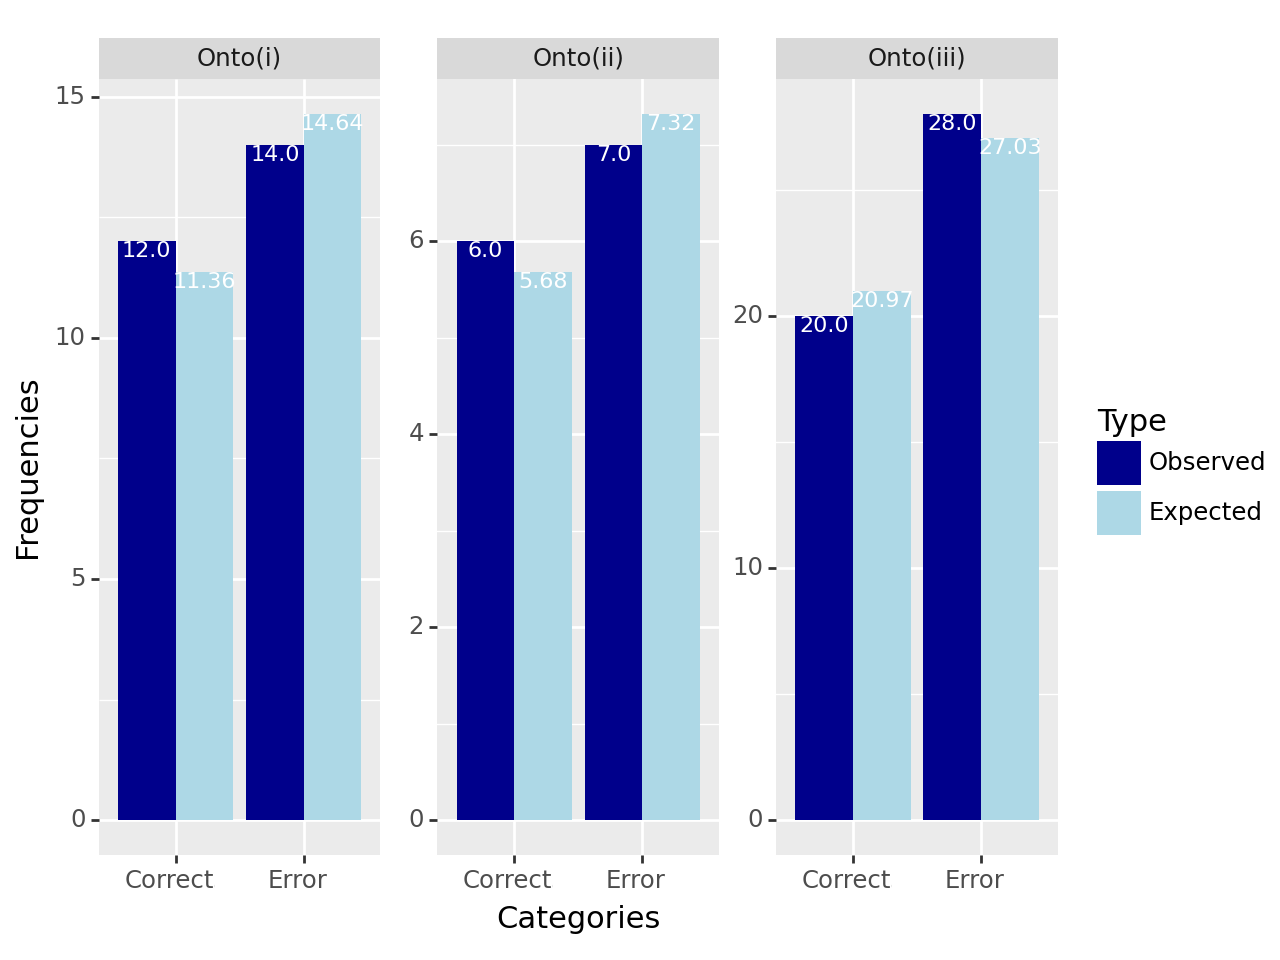
\includegraphics[width=.7\textwidth]{textual/Figuras/Results/Unknown-78.png}
        \caption{ONTO: Observed vs. Expected Frequencies by Meaning (\%).}
        \label{fig: onto-mean-chi}
\end{figure}

\subsubsection{THROUGH by Meaning}

This subsection presents the number of occurrences, correct count, error count, correct rate, and error rate for each meaning of THROUGH. Table~\ref{tab:into-senses} displays this statistics. 

\begin{table}[htb]
\centering
\begin{tabular}{lcccc}
\toprule
 & \multicolumn{4}{c}{\textbf{THROUGH by Meaning}} \\ 
 & \multicolumn{3}{c}{\textbf{SP}} & \textbf{N-SP} \\ 
 & Through(i) & Through(ii) & Through(iii) & Through(v) \\
\midrule
Occurrences & $42$ & $21$ & $70$ & $336$ \\ 
Correct Count & $35$ & $16$ & $50$ & $263$ \\  
Error Count & $7$ & $5$ & $20$ & $73$ \\ 
\midrule
Correct Rate & $\mathbf{83.33\%}$ & $76.19\%$ & $71.42\%$ & $78.27\%$ \\ 
\midrule
Error Rate & $16.66\%$ & $23.80\%$ & $\mathbf{28.57\%}$ & $21.72\%$ \\ 
\bottomrule
\end{tabular}
\caption{THROUGH: Spatial (SP) vs. Non-spatial (N-SP) Counts and Rates by Meaning.}
\label{tab:through-senses}
\end{table}

The analysis of the data in Table~\ref{tab:through-senses} reveals different model performance across the meanings of THROUGH. The highest correct rate, $\approx83\%$, is for ``Through(i)'' which represents ``movement within a passage or conduit''. This suggests that models are particularly accurate in contexts involving clear pathways or conduits. Conversely, the highest error rate, $\approx29\%$, occurs for ``Through(iii),'' which denotes ``movement past or penetrating a barrier'', indicating that models struggle most with scenarios involving this meaning. The ``Through(v)'' category, representing non-spatial usage, shows a correct rate of $\approx78\%$ and an error rate of $\approx22\%$, reflecting moderate accuracy. Overall, the performance varies significantly by meaning, with spatial contexts involving passages being easier for models than those involving barriers.

\subsubsection{$\chi^2$ Test Results for THROUGH by Meaning} 

The Chi-square analysis of the data from Table~\ref{tab:through-senses} yielded a Chi-square statistic of $2.44$ (threshold is $\chi^2 > 7.815$) with a p-value of $0.49$ (threshold is $p < 0.05$) and $3$ degrees of freedom (df). Figure~\ref{fig:through-mean-chi} illustrates the disparities between expected and observed frequencies for the correct and error counts across the different meanings of THROUGH. This indicates that there is no statistically significant difference in the distribution of correct and error counts across the various senses of THROUGH. The high p-value suggests that the observed variation in model performance across different meanings of THROUGH is not statistically significant. Therefore, the differences in correct and error rates do not imply a meaningful disparity in model performance across spatial and non-spatial contexts. This suggests that models perform similarly across these senses, regardless of the specific spatial or non-spatial context.

\begin{figure}[ht]
        \centering
        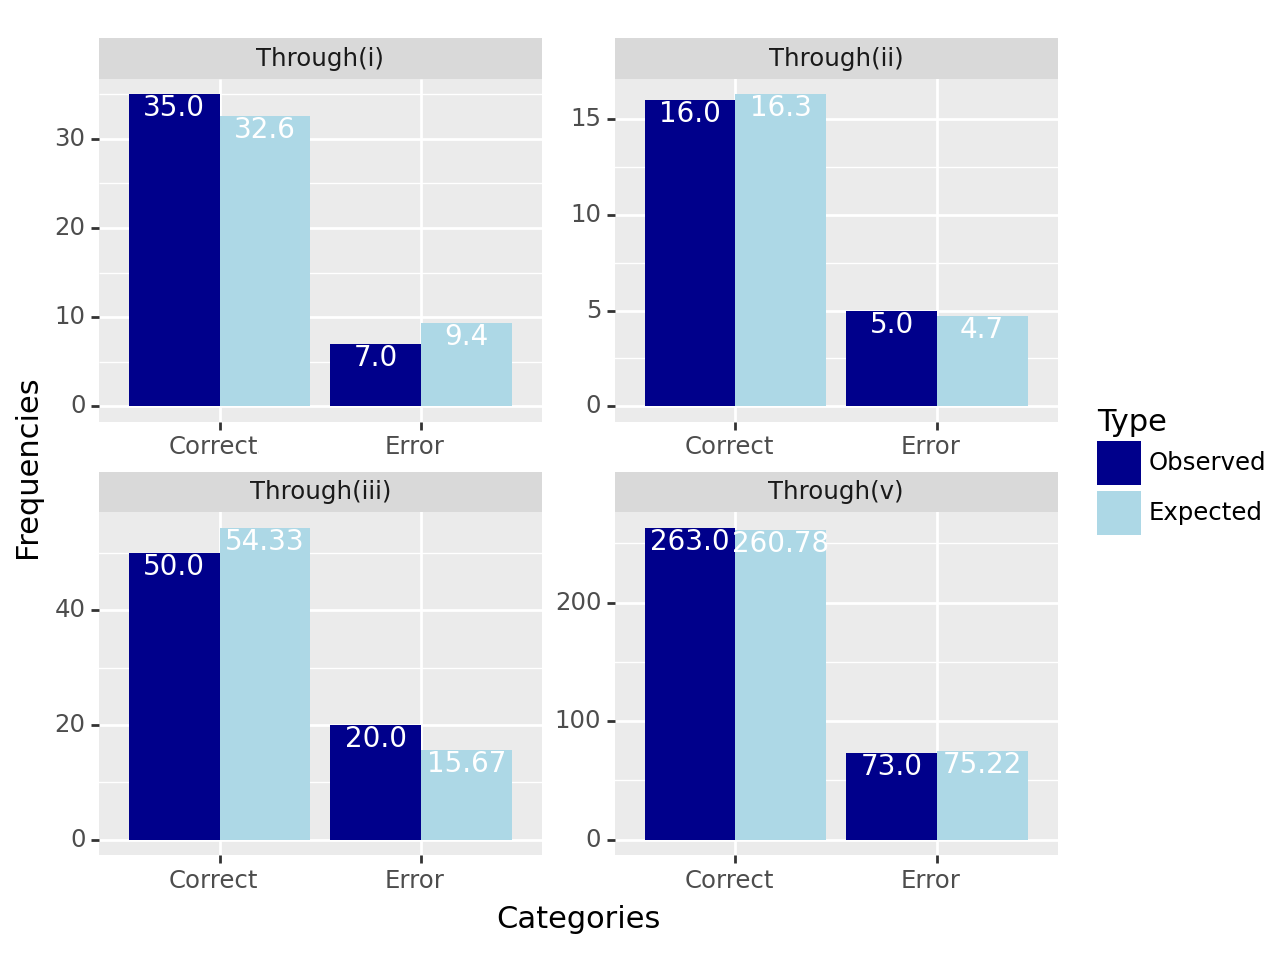
\includegraphics[width=.8\textwidth]{textual/Figuras/Results/Unknown-79.png}
        \caption{THROUGH: Observed vs. Expected Frequencies by Meaning (\%)}
        \label{fig:through-mean-chi}
\end{figure}

\subsubsection{TOTAL} 

In this subsection, we provide the results for the number of occurrences, correct count, error count, correct rate, and error rate across all prepositions. Table~\ref{tab:total} displays the statistics for both spatial and non-spatial categories.

\begin{table}[htb]
\centering
\begin{tabular}{@{}lccc@{}} \\
\toprule
& \multicolumn{2}{c}{\textbf{TOTAL}} \\ 
& \textbf{SP} & \textbf{N-SP} \\
\midrule
Occurrences & $413$ & $987$ \\
Correct Count & $298$ & $787$ \\
Error Count & $115$ & $200$ \\
\midrule
Correct Rate & $72.15\%$ & $\mathbf{79.73\%}$ \\
\midrule
Error Rate & $\mathbf{27.84\%}$ & $20.26\%$ \\
\bottomrule
\end{tabular}
\caption{TOTAL: Spatial (SP) vs. Non-Spatial (N-SP) Observed vs. Expected Frequencies.} \label{tab:total} 
\end{table}

The analysis of Table~\ref{tab:total} indicates a notable difference between non-spatial and spatial senses. Non-spatial senses exhibited a significantly higher number of occurrences ($987$) compared to spatial senses ($413$), as well as a higher correct count ($787$ vs. $298$) and error count ($200$ vs. $115$). However, when considering percentages, non-spatial senses had a considerably higher correct rate ($\approx80\%$ vs. $\approx72\%$) and a lower error rate ($\approx20\%$ vs. $\approx28\%$) compared to spatial senses. This suggests that, while non-spatial senses were more prevalent overall, spatial senses had a higher error rate, indicating a considerably greater challenge in their correct usage.


\subsubsection{$\chi^2$ Test Results for TOTAL} 

The final test yielded a chi-square statistic of $9.168$ and a p-value of $0.0025$ for $1$ degree of freedom (df), both indicating significant results. These values exceed the thresholds of $\chi^2 > 3.841$ for the chi-square critical value and $p < 0.05$ for the p-value, respectively. The results indicate a significant difference between the observed and expected frequencies. The deviations, as illustrated in Figure~\ref{fig:total-chi}, suggest an association between spatial and non-spatial errors and correct responses. Notably, the very low p-value strongly indicates that the observed variations are not due to random chance. This finding implies a meaningful disparity in model performance when considering the total data. Therefore, the distribution of correct and error counts significantly impacts translation accuracy across different prepositions.

\begin{figure}[htb]
        \centering
        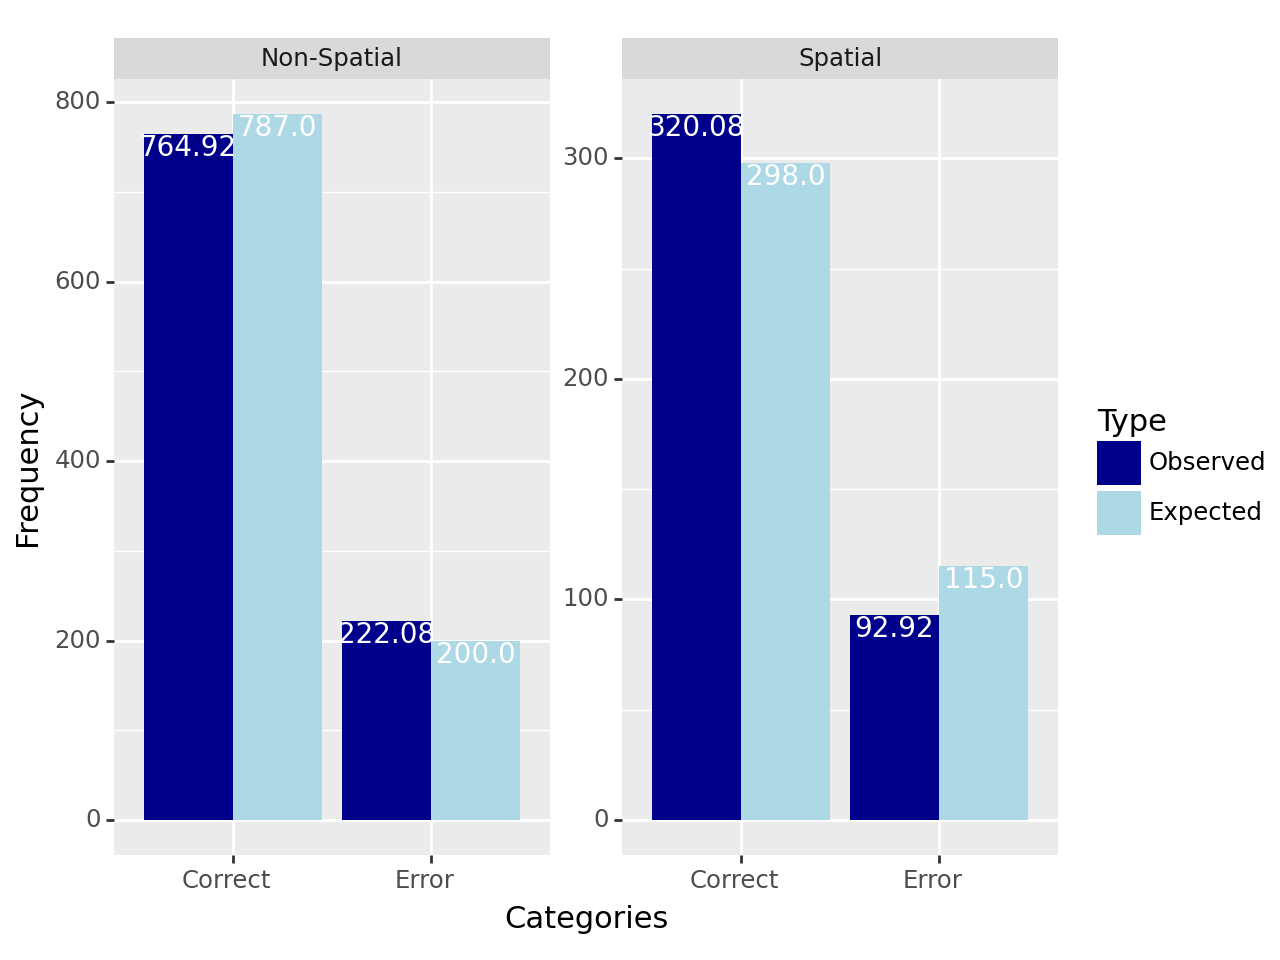
\includegraphics[width=.7\textwidth]{textual/Figuras/Results/Unknown-83.png}
        \caption{TOTAL: Observed vs. Expected Frequencies.}
        \label{fig:total-chi}
\end{figure}

%These findings reiterate our initial proposition that the prevalence of spatial prepositions such as INTO and THROUGH in EN phrasal verbs could potentially influence the larger proportion of ``non-spatial'' errors in our analysis. However, it was interesting to find that, among the spatial senses for INTO and THROUGH, the senses INTO(1) and THROUGH(3) presented the biggest issues during translation. Therefore, we decided to compare that number with the number of sense occurrences in our corpus of 200 segments, and the complete list is in Attachment~\ref{tab:spatial_senses}. We then confirmed that there was indeed a correlation between sense occurrences in the corpus and the issues we found, with INTO(1) having the biggest number number of acorrences among spatial senses (with $23$), followed by THROUGH(3) with $10$ occurrences.

\section{Addressing the Questions and Hypotheses}

In this final subsection, we synthesize the findings from previous sections and revisit out research questions. Specifically, we will respond to questions Q1 and Q2, from Subsection~\ref{sub:q1-q2} of the Introduction. Although we were not able to provide a further quantitative analysis to evaluate the effectiveness of using automated metrics in assessing spatial errors, we will try our best to address questions Q3 and Q4, in Subsection~\ref{sub:q3-q4} qualitatively. Lastly, we will revisit our final chi-square ($\chi^2$) test results from the last subsection to draw meaningful conclusions about our hypotheses. 

\subsection{Accuracy, Fluency, and Post-Editing Needs in LLMs}

When comparing NMTs and LLMs to address Q1, we observe distinct performance patterns in their accuracy, fluency, and post-editing needs. Within the NMT group, performance is fairly consistent. However, within the LLM group, there is considerable variability.

In terms of accuracy, performance variation among LLMs is evident in both BLEU scores, which measure \emph{n}-grams, and METEOR scores, which account for synonyms and aspects such as word order. Notably, certain outliers among LLMs significantly influence performance metrics. Generally, both BLEU and METEOR tend to impose more stringent penalties on translations, highlighting the differences between NMTs and LLMs.

BERTScore and COMET, which are intended to reflect fluency and relevance, present a mixed picture. On one hand, these scores indicate that the confidence intervals (CIs) between some NMTs and LLMs overlap, suggesting a margin for similar performance between the two groups. On the other hand, these scores show the least clarity when relied on for ranking model performance, especially BERTScore, as they sometimes assign high scores to translations that human evaluations judged to be poor (see Example~\ref{ex:14}).

\ex.\texttt{(inner\_id: 7038)} \hfill  \texttt{Across(ii)} \\[0.3ex] \label{ex:ex-14}
\noindent\rule{\linewidth}{0.9pt}
Local communities on the East Coast \textcolor{blue}{would get together} and whole teams of 10, 20 people would \colorbox{lightblue}{\textcolor{blue}{caravan}}  \colorbox{lightgray}{\textcolor{blue}{\emph{across}}} the United States, and they would form companies. (SRC) \\[0.3ex]
\noindent\rule{\linewidth}{0.3pt}
Pequenas comunidades do Leste \textcolor{ForestGreen}{se uniriam} em equipes de 10 ou 20 pessoas e \colorbox{lightgray}{\textcolor{ForestGreen}{\emph{atravessariam}}} o país, e formariam empresas.  (REF) \\[0.3ex]
\noindent\rule{\linewidth}{0.3pt}
As comunidades locais na costa Leste \textcolor{ForestGreen}{se reuniam} e formavam grupos inteiros de 10 ou 20 pessoas, que \colorbox{lightgray}{\textcolor{ForestGreen}{\emph{cruzariam}}} os Estados Unidos \colorbox{lightblue}{\textcolor{ForestGreen}{em caravanas}} e fundariam empresas. (Gemma-7B) \\[0.3ex]
\noindent\rule{\linewidth}{0.3pt}
?~As comunidades locais no litoral do Leste dos Estados Unidos \textcolor{Maroon}{se juntam} e equipes de 10 ou 20 pessoas \colorbox{lightblue}{\textcolor{Maroon}{caravaneiam}} \colorbox{lightgray}{\textcolor{Maroon}{\emph{através}}} dos Estados Unidos \textcolor{Maroon}{inteiros}, formando empresas. (LLaMa-2-7B)  \\[0.3ex]
\noindent\rule{\linewidth}{0.3pt}
?~Comunidades locais na Costa Leste \textcolor{ForestGreen}{se reuniam} e equipes inteiras de 10 a 20 pessoas \colorbox{lightblue}{\textcolor{Maroon}{faziam piqueniques transcontinentais}} nos EUA, e elas formavam empresas. (LLaMa-3-8B)  \\[0.3ex]
\noindent\rule{\linewidth}{0.3pt} 
?~Comunidades locais na Costa Leste \textcolor{ForestGreen}{se reuniam} e equipes inteiras de 10, 20 pessoas \colorbox{lightblue}{viajavam em \textcolor{Maroon}{caravana}} \colorbox{lightgray}{\textcolor{Maroon}{\emph{através}}} dos Estados Unidos e formavam empresas. (Mixtral-8x7B) \\[0.3ex]
\noindent\rule{\linewidth}{0.9pt}


\begin{table}[htb]
\centering
\begin{tabular}{@{}lccccc@{}}
\toprule
& \multicolumn{5}{c}{\textbf{MT Metric}} \\
\textbf{Model} & \textbf{BLEU} & \textbf{METEOR} & \textbf{BERTScore} & \textbf{COMET} & \textbf{TER} \\
\midrule
Gemma-7B & $0.008$ & $0.087$ & $0.396$ & $0.697$ & $130.0$ \\
LLaMa-2-7B & $\mathbf{0.213}$ & $\mathbf{0.589}$ & $0.958$ & $0.772$ & $80.0$ \\
LLaMa-3-8B & $0.035$ & $0.512$ & $\mathbf{0.976}$ & $0.777$ & $\mathbf{75.0}$ \\
Mixtral-8-7B & $0.034$ & $0.537$ & $0.973$ & $\mathbf{0.797}$ & $85.0$ \\
\bottomrule
\end{tabular}
\caption{MT Metrics for the Translation in Example (14).}
\label{tab:final}
\end{table}

Example~\ref{ex:ex-14} illustrates a scenario where automatic metrics exhibited significant disparities in evaluating translations from different models, resulting in compromised model assessment. Beginning with Gemma-7B, which produced a correct (cc) translation, we observed no issues. The only deviations from the reference (REF) were the use of a synonym, ``cruzariam,'' instead of ``atravessariam,'' to convey the Path (moving transversally) and the expression of the Manner component through the adjunct ``em caravanas,'' which aligns perfectly with the expected lexicalization patterns of motion expression in \texttt{verb-framed} language PT-br \parencite{talmy1985lexicalization, talmy2000towardb, slobin2005relating, oliveira2022expressing}. However, its scores, particularly BLEU ($0.008$), METEOR ($0.087$), and BERTScore ($0.396$), were notably low compared to other models (see Table~\ref{tab:final} for a comparison). In addition, the very high TER score ($120.0$), indicating the need for 120 edits to align with the reference, further emphasizes this discrepancy.

LLaMa-2-7B, however, exhibited a syntactic projection (sp) error and an interlanguage/code-switching (in) error with the combination ``caravaneiam através (de),'' as ``caravanear'' is not dictionary-registered or even a lexicalized term in PT-br. Additionally, ``se juntam'' contained a wrong tense/mood (wt) error, and ``inteiros'' was a grammar (gr) error caused by wrong word order. Despite these issues, the translation achieved a considerably high BERTScore ($0.95$). However, BLEU penalized it greatly ($0.21$), METEOR provided a balanced score ($0.58$), and COMET indicated reasonable fluency and relevance ($0.77$). Nonetheless, a TER of $80.0$ highlighted significant post-editing needs.

Similarly, LLaMa-3-8B, demonstrated a case of wrong lexical choice (wl) with the phrase ``faziam piqueniques transcontinentais,'' which has nothing to do with ``caravan across''. This translation indicates a complete mistranslation of the source text. In contrast, Mixtral-8-7B provided ``viajaram em caravana através (de),'' which presents a wrong sense (ws) issue. While ``viajaram em caravanas" is an acceptable translation emphasizing the Manner of traveling, ``através (de)'' does not constitute one of the meanings of ACROSS \parencite{McCleary-Viotti-2004}, which, in this context implies moving from one end to the other. Despite these issues, LLaMa-3-8B achieved a considerably high BERTScore ($0.976$), whereas Mixtral-8-7B obtained a considerably high COMET score ($0.797$).

Nevertheless, when ranking models based on their fluency and accuracy, a clear hierarchy emerges. The NMTs DeepL, Amazon, and Google occupy the top tier in that order. Among LLMs, LLaMa-3-8B and Mixtral-8-7B show the highest fluency and accuracy, performing well to a certain extent. Surprisingly, Gemma-7B, despite being heavily penalized in automated scores, performs reasonably well in human evaluations. Lastly, the other LLMs—LLaMa-2-13B, LLaMa-2-7B, and Mistral-7B, respectively, show the lowest performance compared to the top LLMs. This performance ranking highlights that the relationship between the model architecture, the number of parameters, and their performance is not always strictly linear. For instance, Gemma-7B, with only 7 billion parameters, slightly outperforms LLaMa-2-13B, which has 13 billion parameters.

In addressing questions Q3 and Q4, we can draw insights from the performance metrics used to evaluate translations involving spatial prepositions (ACROSS, THROUGH, INTO, and ONTO) from EN-PT-br. The effectiveness of widely-used evaluation metrics like BLEU, METEOR, BERTScore, COMET, and TER varies significantly in capturing accuracy and penalizing spatial errors in translations. In general, BLEU tends to penalize translations heavily, especially for differences in grammatical structure, and its scores are hard to interpret. Conversely, METEOR is less strict, using stemming and considering synonyms from databases as described by~\textcite{koehn2020neural}, but in this case, it overlooked the synonyms ``atravessar'' and ``cruzar'' in PT-br. BERTScore struggles with differentiating between incorrect translations that closely resemble the reference and more accurate ones with different wording, especially when stylistically similar \parencite{hanna-bojar-2021-fine}, which is exactly what we encountered in Example~\ref{ex:ex-14}. COMET often faces issues such as missing named entities, omissions of content, and unnecessary insertions \parencite{glushkova2023bleu}; although we did not identify those in our analysis, we did notice a tendency to still attribute a relatively high score to translations resembling the source. Lastly, TER provides an indication of the number of edits required for alignment with the reference, quantifying post-editing needs, but understanding which edits are considered can be challenging due to their volume, making interpretation difficult.

Moreover, post-editing was not required for NMT systems, but it was highly necessary for LLMs, although to varying degrees. Some LLMs necessitated less post-editing than others, with Mistral-7B needing the most. Even with the alternative prompt specifying the exclusion of unnecessary information, Mistral-7B's outputs required significant post-processing compared to other LLMs. See Example~\ref{ex:ex15} for an illustration.

\ex.\texttt{(inner\_id: 2797)} \hfill  \texttt{Into(iii)}\\[0.3ex] \label{ex:ex15}
\noindent\rule{\linewidth}{0.9pt}
But here's the thing: our aim is to encourage students to articulate their own opinions, not to coerce them \colorbox{lightgray}{\emph{into}} agreeing with us, so it actually doesn't matter if he and I agree. (SRC) \\[0.3ex]
\noindent\rule{\linewidth}{0.3pt}
Mas, penso da seguinte forma, nosso objetivo é incentivar os alunos a articular opiniões próprias, e não coagi-los \colorbox{lightgray}{\emph{a}} concordar conosco. Por isso, não importa se eu e ele concordarmos. (REF)\\[0.3ex]
\noindent\rule{\linewidth}{0.3pt}
\colorbox{lightyellow}{\textcolor{Maroon}{Eu sou um profissional de tradução. Traduzir o texto seguinte em Português}}\\ Mas aqui está a coisa: nossa intenção é encorajar estudantes a articular suas próprias opiniões, não forçá-los \colorbox{lightgray}{\emph{a}} concordar \colorbox{lightgray}{\textcolor{Maroon}{com nós}}, então realmente não importa se ele e eu concordamos. \colorbox{lightyellow}{\textcolor{Maroon}{(Translation: "But here's the thing: our aim is to}}  \colorbox{lightyellow}{\textcolor{Maroon}{encourage students to articulate their own opinions, not to coerce them into}}\\ \colorbox{lightyellow}{\textcolor{Maroon}{agreeing with us, so itactually doesn't matter if he and I agree.")}} (Mistal-7B) \\[-0.3ex] 
\noindent\rule{\linewidth}{0.9pt}

In general, a clear observation arises. Open-source LLMs tend to generate extensive additional content, which is often redundant or irrelevant to the task. As seen in Example~\ref{ex:15}, Mistral-7B's outputs required the most post-processing among the LLMs we explored, necessitating the removal of source sentences and other extraneous information. The post-editing efforts varied significantly among different systems, highlighting the importance of optimizing LLMs for practical use in translation tasks.


\subsection{Most Prevalent Spatial Prepositions, Meanings, and Errors}

At the core of our research was understanding which spatial prepositions and meanings pose particular challenges for LLMs and NMTs in translation tasks. Question Q2 specifically examines the prevalence of spatial errors -- polysemy (po), syntactic projection (sp), and wrong sense (ws) -- and their impact on translation quality. To address this question, we analyzed the top five meanings with the highest spatial error rates from Figure~\ref{fig: all-perc}.

Table~\ref{tab:finall} summarizes the findings, highlighting the most prevalent prepositions, their meanings, and the most frequently encountered spatial errors. We focused specifically on the senses with the highest error proportions by preposition, as identified in Figure~\ref{fig: all-perc} in Subsection~\ref{subsec: sp-vs-nsp}. As observed, the prepositions ACROSS, THROUGH, and INTO each showed one or more senses with a notably higher proportion of spatial errors. However, the preposition ONTO was excluded from the analysis, as its two spatial meanings, Onto(i) and Onto(ii), exhibited the same percentage of errors ($14\%$), indicating no particular prominence in either prepositional sense or spatial error. This analysis identifies patterns and areas for improvement in handling spatial language within translation models.

\begin{table}[htb]
\centering
\begin{tabular}{@{}llccccccccc@{}}
\toprule
& & \multicolumn{6}{c}{\textbf{Spatial Errors}} \\
\cmidrule(lr){3-8}
& & \multicolumn{2}{c}{\textbf{po}} & \multicolumn{2}{c}{\textbf{sp}} & \multicolumn{2}{c}{\textbf{ws}} \\
\cmidrule(lr){3-4} \cmidrule(lr){5-6} \cmidrule(lr){7-8}
\textbf{Preposition} & \textbf{Meaning} & \textbf{Count} & \textbf{\%} & \textbf{Count} & \textbf{\%} & \textbf{Count} & \textbf{\%} \\
\midrule
\multirow{1}{*}{ACROSS} & Across(ii) & $1$ & $5.5\%$ & $\mathbf{15}$ & $83.3\%$ & $5$ & $27.7\%$ \\
\multirow{2}{*}{INTO} & Into(ii) & $2$ & $11.7\%$ & $\mathbf{6}$ & $35.2\%$ & $1$ & $5.8\%$ \\
& Into(i) & $19$ & $28.7\%$ & $\mathbf{26}$ & $39.3\%$ & $1$ & $1.5\%$ \\
\multirow{2}{*}{THROUGH} & Through(iii) & $2$ & $10.5\%$ & $\mathbf{17}$ & $89.4\%$ & $1$ & $5.2\%$ \\
& Through(ii) & $1$ & $16.6\%$ & $\mathbf{3}$ & $50\%$ & $1$ & $16.6\%$ \\
\bottomrule
\end{tabular}
\caption{Most Prevalent Prepositions, Meanings, and Spatial Errors: Counts and Rates (\%).}
\label{tab:finall}
\end{table}


The data in Table~\ref{tab:finall} indicates that syntactic projection (sp) errors, followed by polysemy (po), were the most prevalent across the spatial prepositions analyzed in our study. For instance, the preposition ACROSS with the meaning ``Across(ii) -- movement over a surface,'' has $15$ syntactic projection errors, accounting for $83.3\%$ of the errors in this category. Conversely, polysemy (po) and wrong sense (ws) errors account for $5.5\%$ and $27.7\%$, respectively. Similarly, for the preposition INTO with the meaning ``Into(ii) -- movement resulting in contact or collision,'' there are $6$ syntactic projection (sp) errors, representing $35.2\%$ of the total errors. Polysemy (po) and wrong sense (ws) errors represent $11.7\%$ and $5.8\%$, respectively, for this meaning. Additionally, the meaning ``Into(i) -- movement or direction leading to enclosure,'' there are $26$ syntactic projection errors ($39.3\%$), with polysemy and wrong sense errors accounting for $28.7\%$ and $1.5\%$, respectively. For THROUGH with the meaning ``Through(iii) -- movement past or penetrating a barrier,'' there are $17$ syntactic projection errors ($89.4\%$), with polysemy and wrong sense errors at $10.5\%$ and $5.2\%$, respectively. Lastly, for THROUGH with the meaning ``Through(ii) -- movement within an open area, region, or place,'' there are $3$ syntactic projection errors ($50\%$), and polysemy and wrong sense errors at $16.6\%$ each.

These findings underscore the significant challenge posed by syntactic projection (sp) and polysemy (po) errors in both LLMs and NMTs. Our analysis reveals that spatial semantics indeed influences NMT as a whole, independent of specific groups. When examining the occurrence counts in Table~\ref{tab:model_performance_by_error_type}, we observe that LLMs exhibited a considerably higher count of spatial errors compared to DeepL. However, the proportion of these errors within DeepL's translations was drastically significant, accounting for 35\% (2-5 times more than LLMs) of errors. This indicates that spatial semantics is a pervasive issue affecting NMT overall, although open-source untuned LLMs might be considerably more prone to these errors, due to their propensity for translation errors in general.

Moreover, the final results of the chi-square ($\chi^2$) test refute the null hypothesis of independence, negating the assumption that spatial semantics does not influence NMT performance. The significant correlation between spatial and non-spatial errors and translation quality emphasizes the importance of addressing the inherent challenges of spatial language, including preposition polysemy \parencite{coventry:04b, herskovits1986language} and language typology \parencite{talmy2000towardb, McCleary-Viotti-2004, slobin2005relating, cadierno2017thinking, oliveira2022expressing}, as well as the nuanced semantics of idiomatic expressions. These findings suggest that, at least for the models we analyzed, while ``decoder-only'' open-source LLMs show great promise, established NMT systems, with their ``encoder-decoder'' transformer architecture might still offer a superior performance for translation tasks due their ability to handle sequential generation more effectly and tailored training on large parallel  datasets \parencite{lakew2019multilingual, koehn2020neural}.






